\label{ch:database}

This chapter investigates different methods to accelerate the delayed heating calculation for experiments of arbitrary material composition.
The most computationally expensive step in the delayed heating calculation is the neutron-transport simulation during experiment irradiation.
This step determines the geometry-dependent parameters, i.e., total neutron flux, neutron spectrum, and reaction rates.
Section \ref{sec:fast} introduces a \textit{fast calculation} method and investigates the possibility of avoiding the repeated run of the neutron-transport simulation to save on computational resources.

Based on the fast calculation results, Section \ref{sec:irradatabase} introduces the \textit{Generic Irradiation Database} method and discusses the results of two applications.
The first application verifies the generic material irradiation database method for the simple demonstration exercise introduced in Section \ref{sec:demo}.
The second application is the verification of the method for an ATR experiment.

\section{Fast Calculation}
\label{sec:fast}

This method solves the neutron-transport problem only once for a specific experiment material to obtain the geometry-dependent parameters.
Then, these parameters are fixed and become the input to the rest of the delayed heating calculation workflow regardless of the experiment composition.
The depletion calculation utilizes these fixed parameters to obtain the charged particle heating and photon source intensity.
The method underlying assumption is that the experiment volume is small enough to perturb the neutron flux in the reactor, and that for all experiment materials the neutron flux is approximately the same.
% As shown in Figure \ref{fig:atr-flux}, the total neutron flux in experiments of different chemical elements is bounded between 3.4 to 6.0 $\times$ 10$^{14} n/cm^2/s$.
As shown in Figure \ref{fig:atr-flux}, the total neutron flux in experiments of different chemical elements is bounded between 3.2 to 5.1 $\times$ 10$^{14} n/cm^2/s$.
These results show that the total neutron flux in the experiment does not vary strongly and always remains in the same order of magnitude.
As the first step of the delayed heating calculation obtains the neutron flux, fixing its value within the range shown in the figure may allow for a sufficiently accurate delayed heating calculation.

\begin{figure}[htbp!]
  \begin{center}
    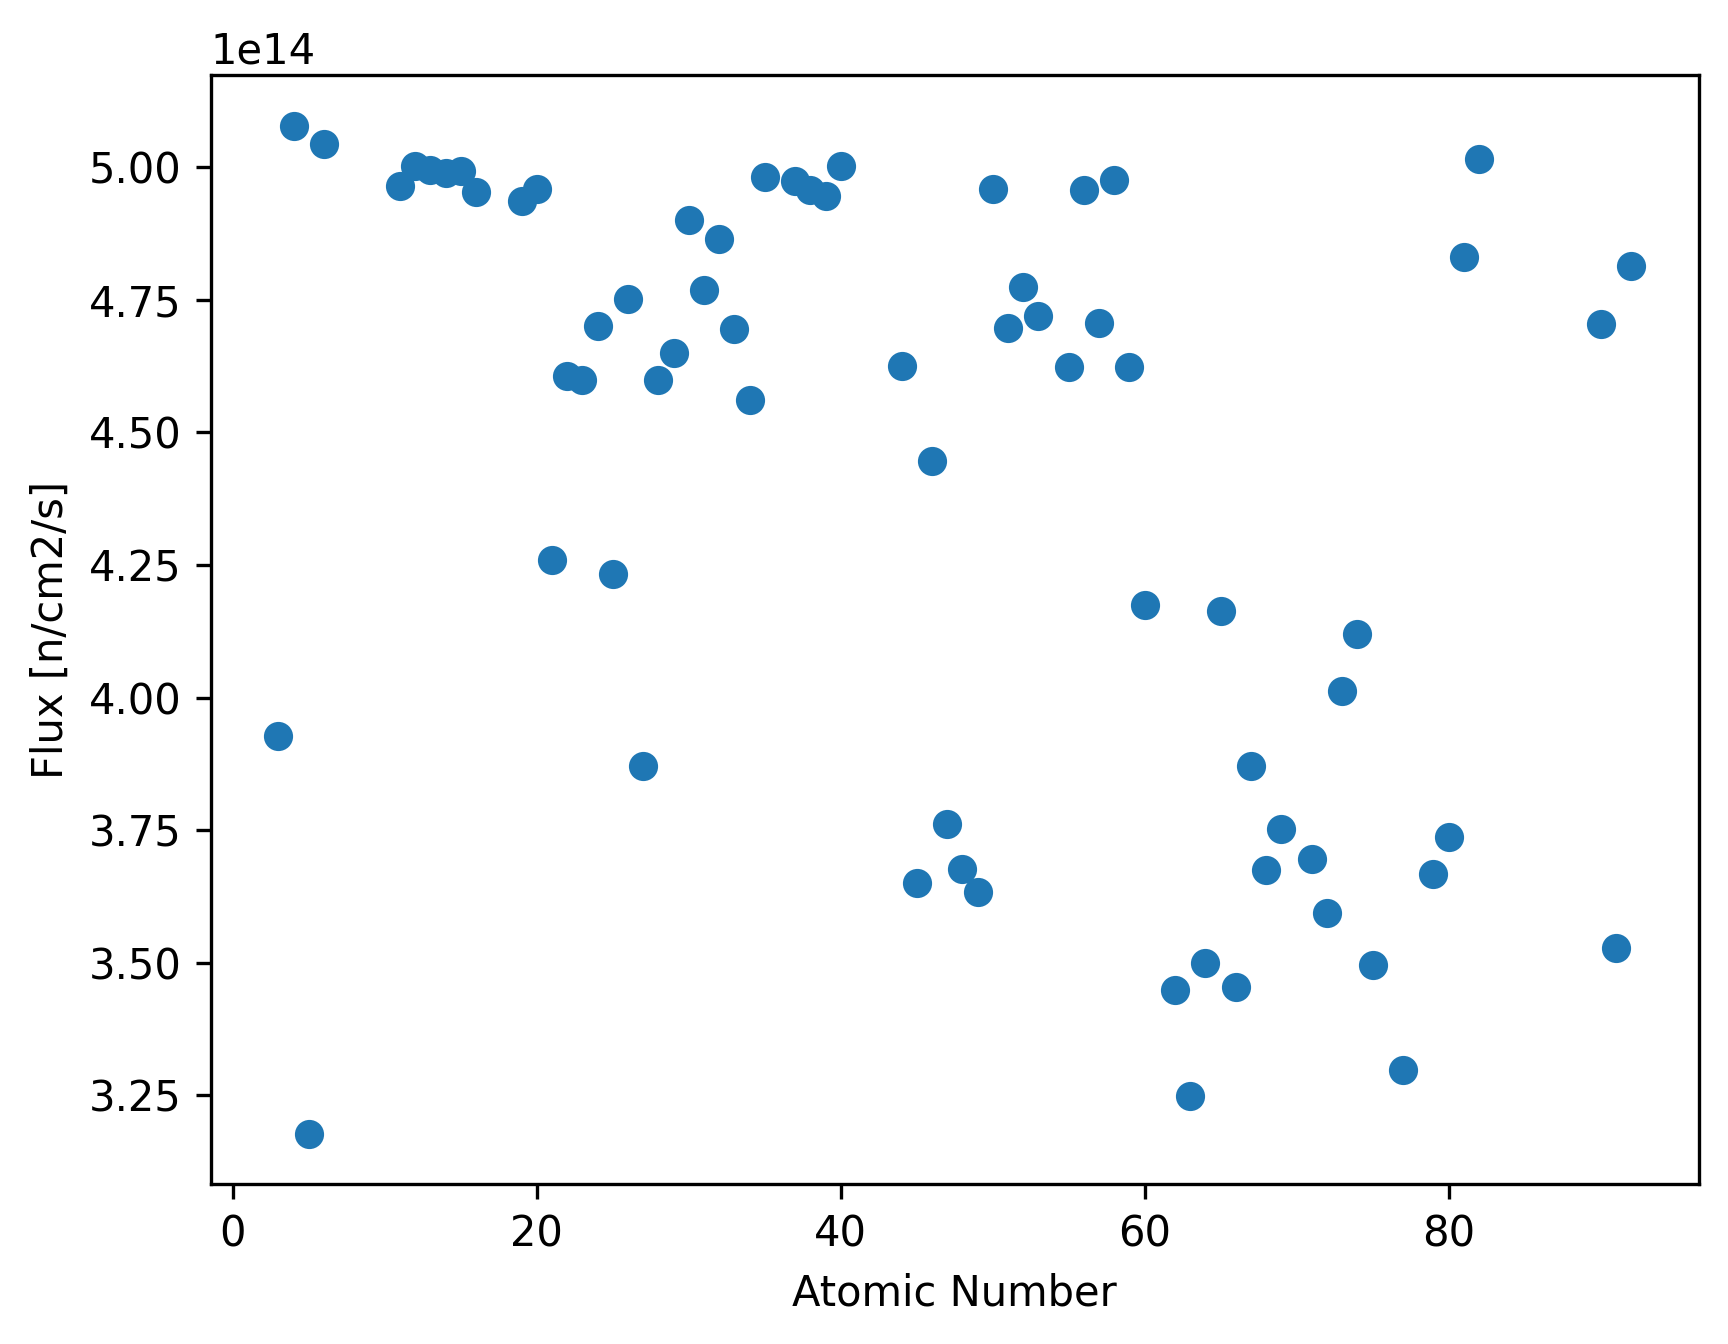
\includegraphics[width=0.60\linewidth]{figures/demo-materials-flux}
  \end{center}
  \caption{Total neutron flux vs. atomic number of the experiment material.}
  \label{fig:atr-flux}
\end{figure}

As the neutron-transport simulation must be run at least once to fix the geometry-dependent parameters, the question that remains unanswered is what experiment material should be chosen for the simulation.
Two materials are studied: one that considerably perturbs the flux, which is 20\%-enriched uranium, and one that barely perturbs the flux, which is carbon.
Although not shown here, when utilizing the geometry-dependent parameters from the neutron-transport simulation for an experiment of uranium, the delayed heating results are not accurate.
That is because perturbing the reactor flux to obtain the fixed geometry-dependent parameters is not desirable as originally expected.
When perturbing the flux, as the reactor power remains constant, the flux in the experiment increases, while the flux in the fuel assemblies decreases.
Hence, the fuel assemblies are subject to a lower depletion, and consequently they produce a lower delayed gamma emission rate.
As a result, choosing carbon as the experiment material is more favorable because it does not considerably perturb the flux.

To better understand the effects of the geometry-dependent parameters on the delayed heating, this section presents a sensitivity analysis on some key magnitudes in the calculation workflow, i.e., the energy deposited by charged particles ($H_{ch}$) and the photon emission rate ($S_i$).
The calculations use the demonstration exercise from Section \ref{sec:demo}.
The reference calculation is based on the delayed heating calculation workflow for an  experiment of arbitrary material, while the fast calculation uses the values from the neutron-transport simulation for the experiment of carbon.
Figures \ref{fig:sens-al} to \ref{fig:sens-w} show a sensitivity analysis of the $H_{ch}$ and $S_i$ for different total flux levels and selected experiment materials.
These results show that the fast calculation overestimates the results for all cases.
The overestimation for the experiment of aluminum is minimal, while the overestimation for other cases, such as the experiment of enriched uranium, is relatively large.

\begin{figure}[htbp!] % or H
  \centering
  \begin{subfigure}[b]{0.49\textwidth}
    \centering
    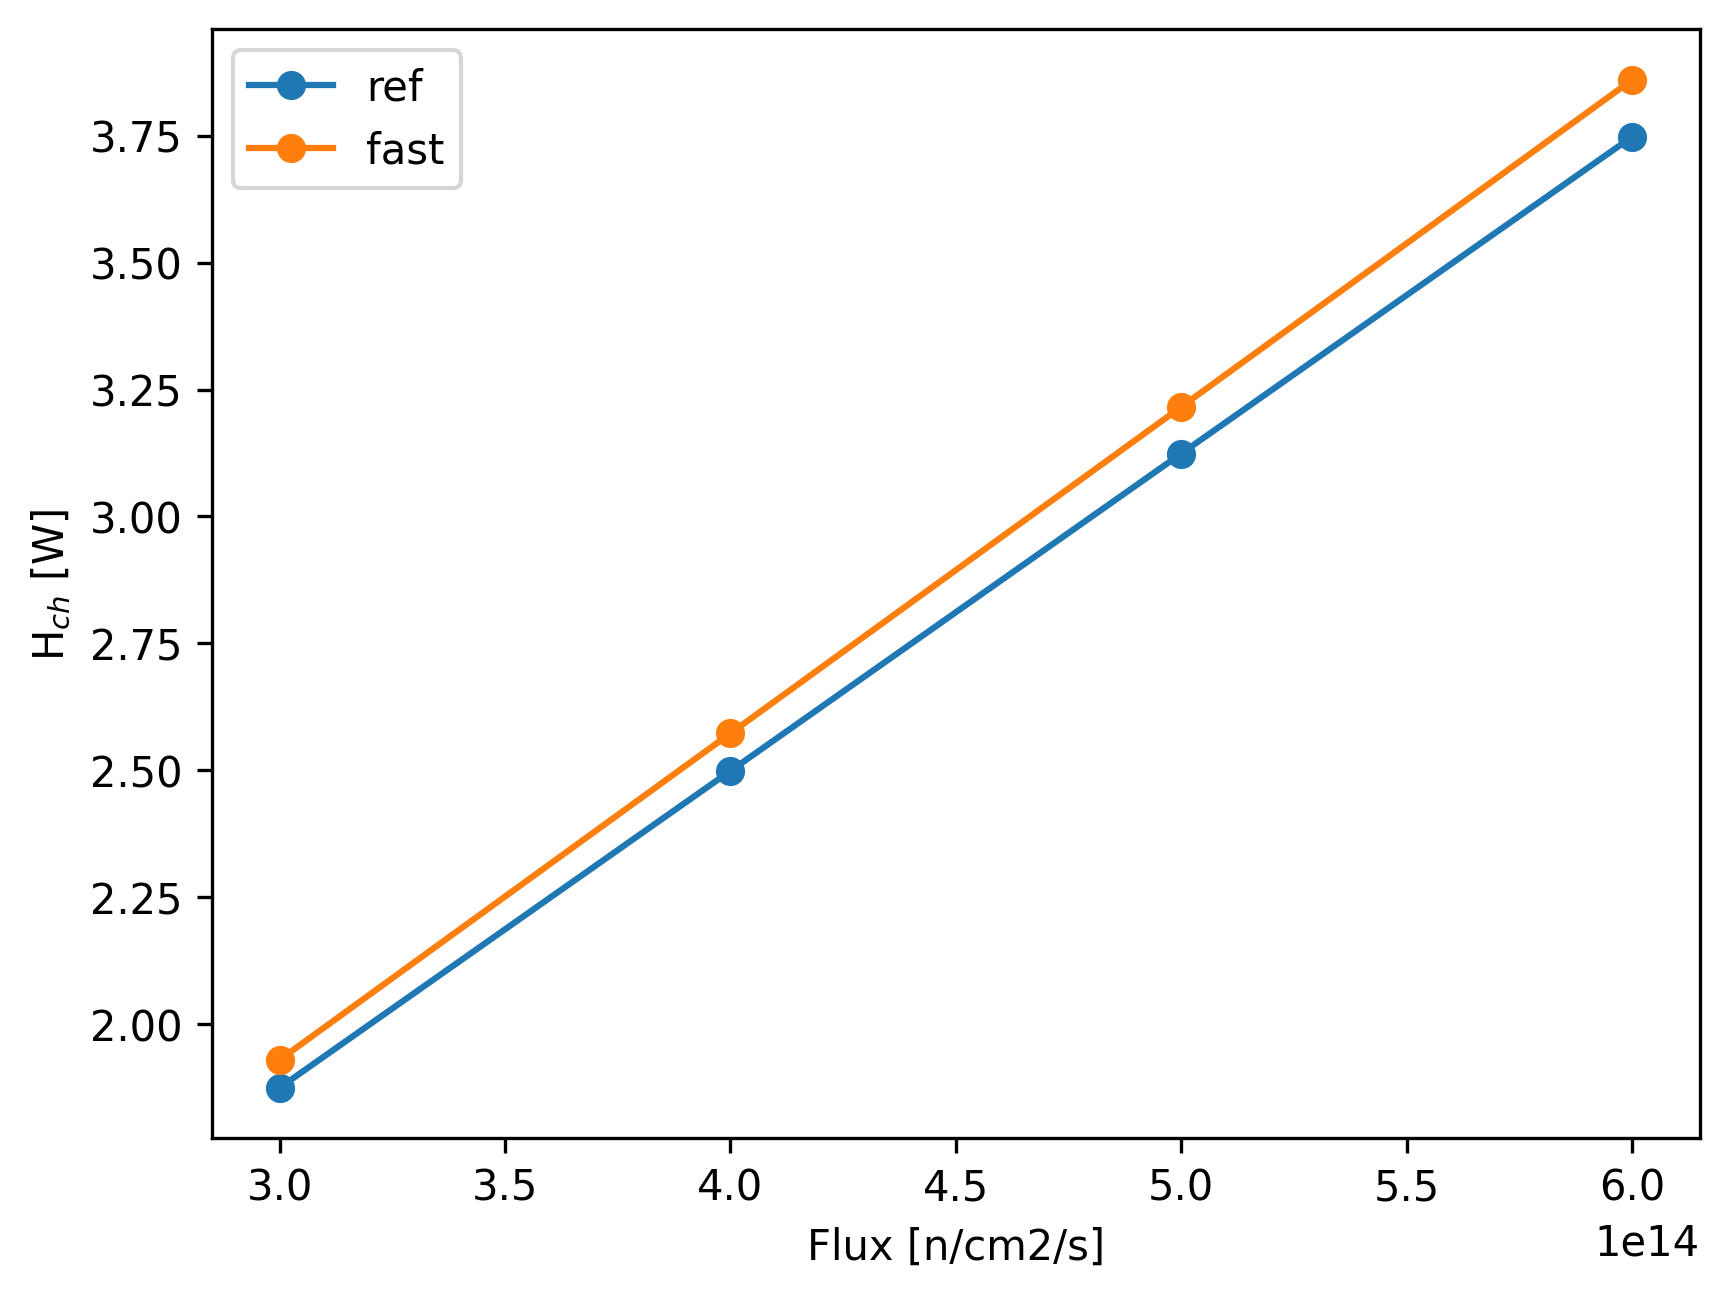
\includegraphics[width=0.7\textwidth]{figures/fast-res13_hch}
    \caption{Energy deposited by charged particles.}
  \end{subfigure}
  \hfill
  \begin{subfigure}[b]{0.49\textwidth}
    \centering
    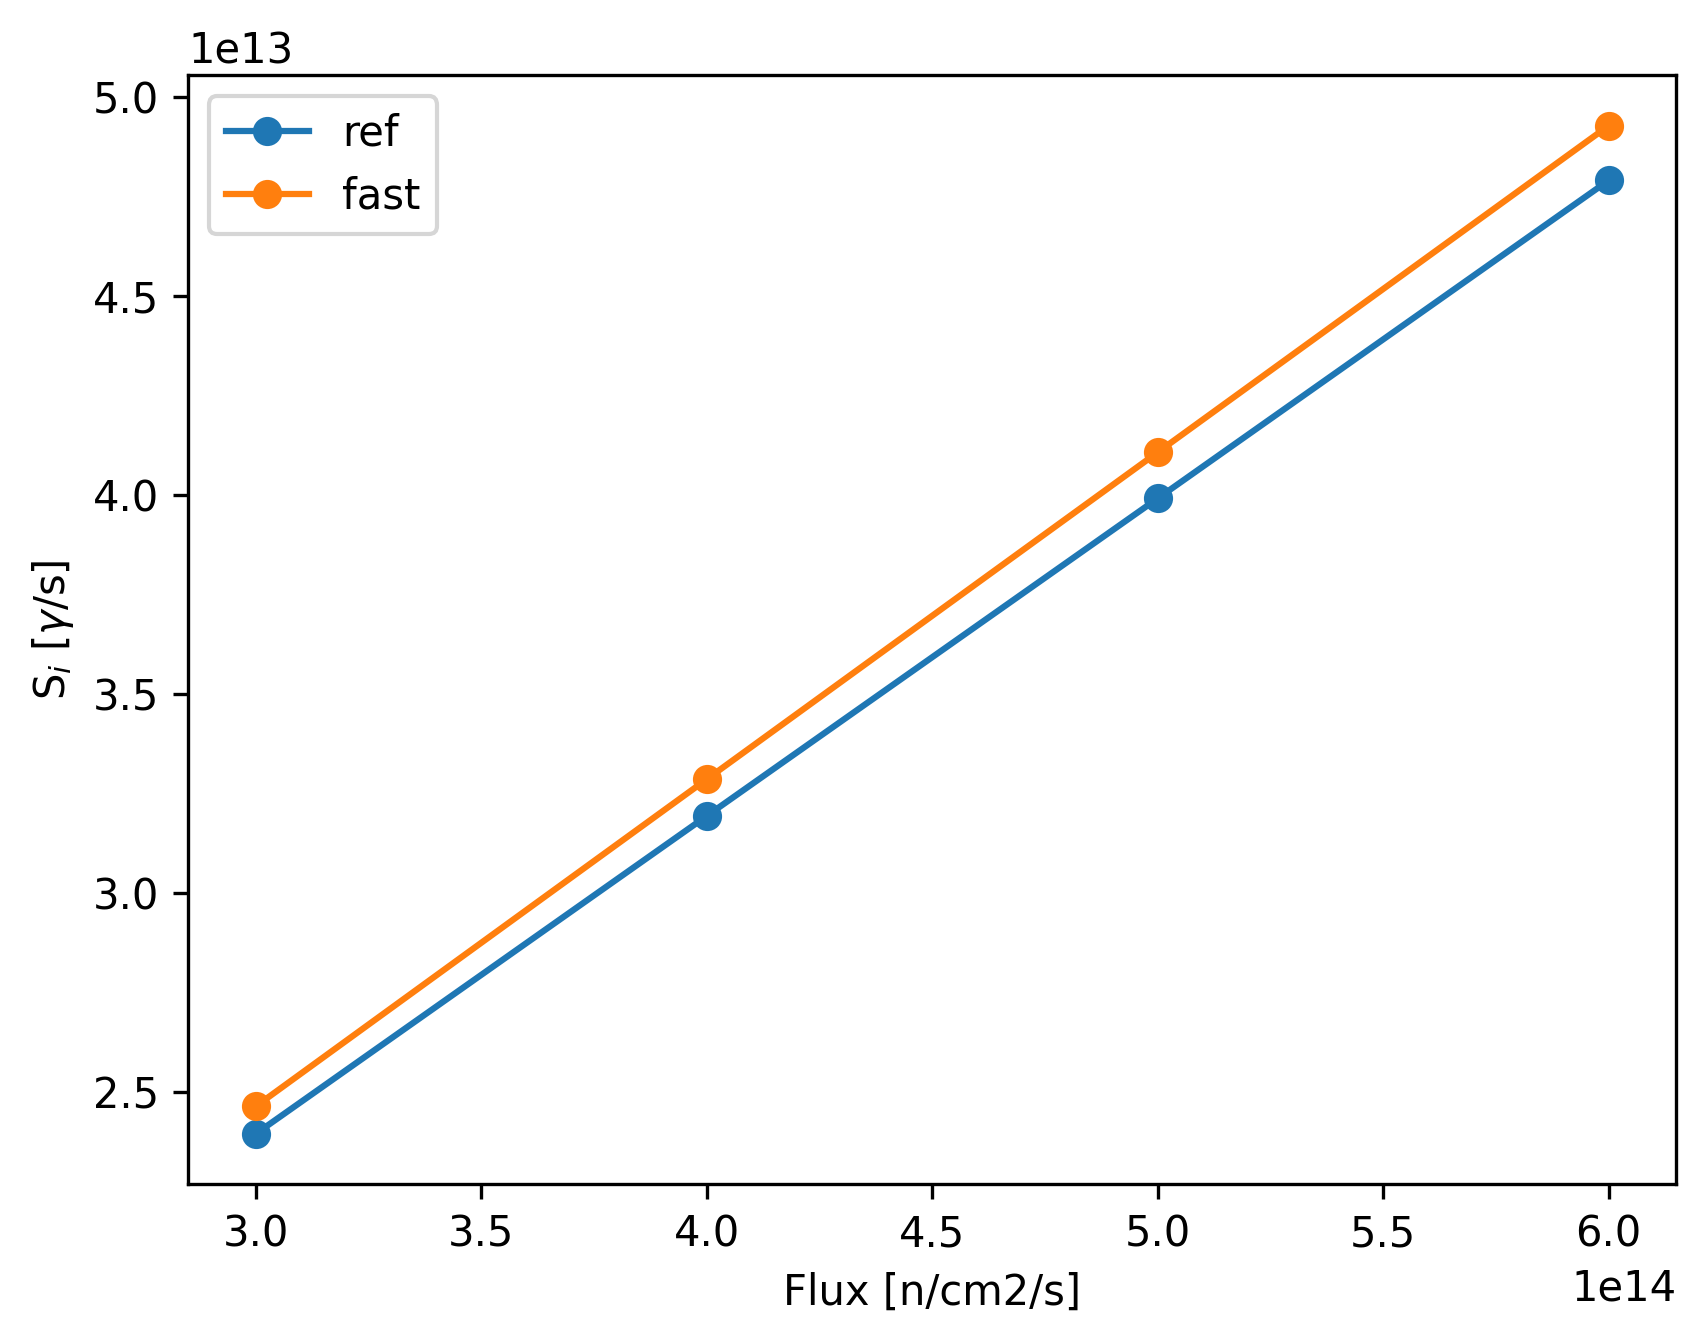
\includegraphics[width=0.7\textwidth]{figures/fast-res13_Si}
    \caption{Photon emission rate.}
  \end{subfigure}
  \hfill
  \caption{Sensitivity analysis for aluminum.}
  \label{fig:sens-al}
\end{figure}

\begin{figure}[htbp!] % or H
  \centering
  \begin{subfigure}[b]{0.49\textwidth}
    \centering
    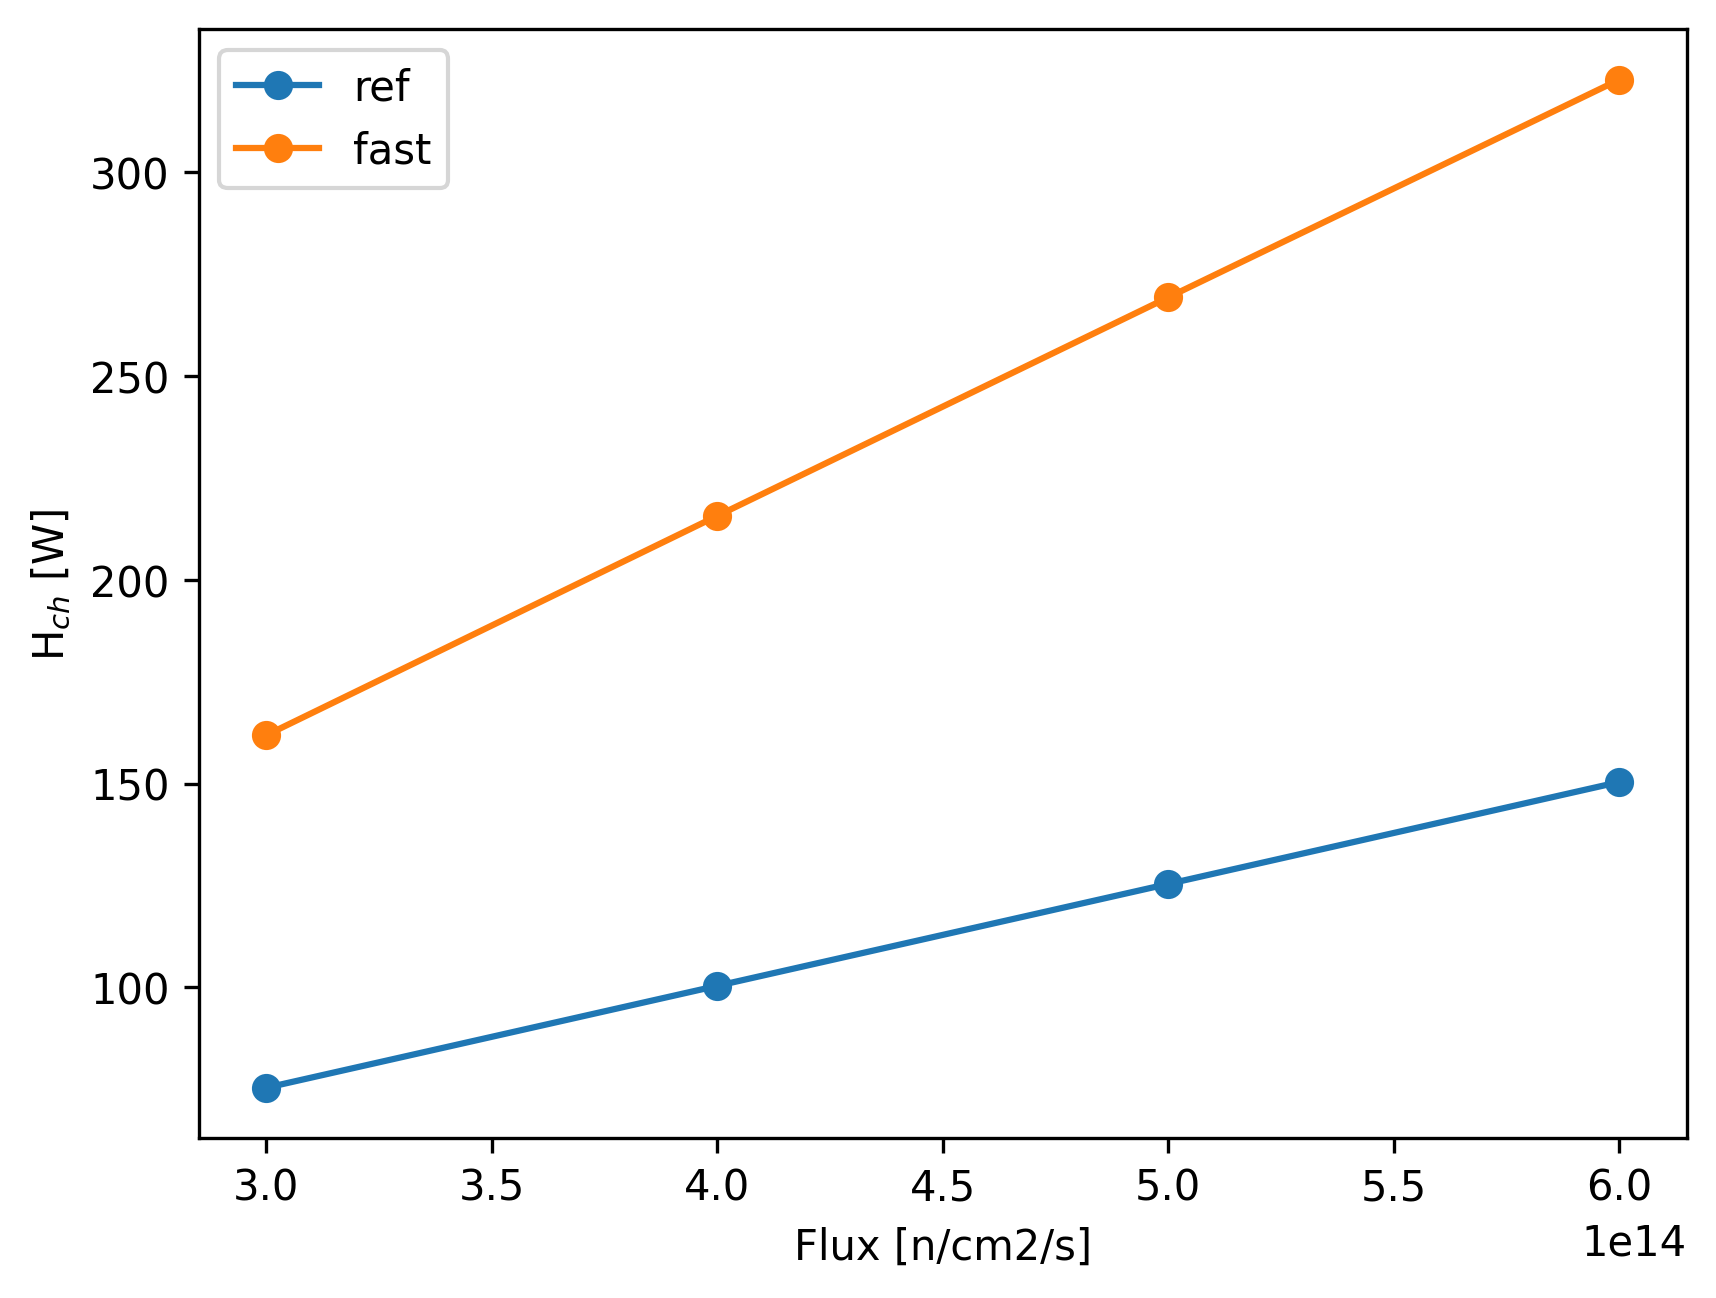
\includegraphics[width=0.7\textwidth]{figures/fast-res25_hch}
    \caption{Energy deposited by charged particles.}
  \end{subfigure}
  \hfill
  \begin{subfigure}[b]{0.49\textwidth}
    \centering
    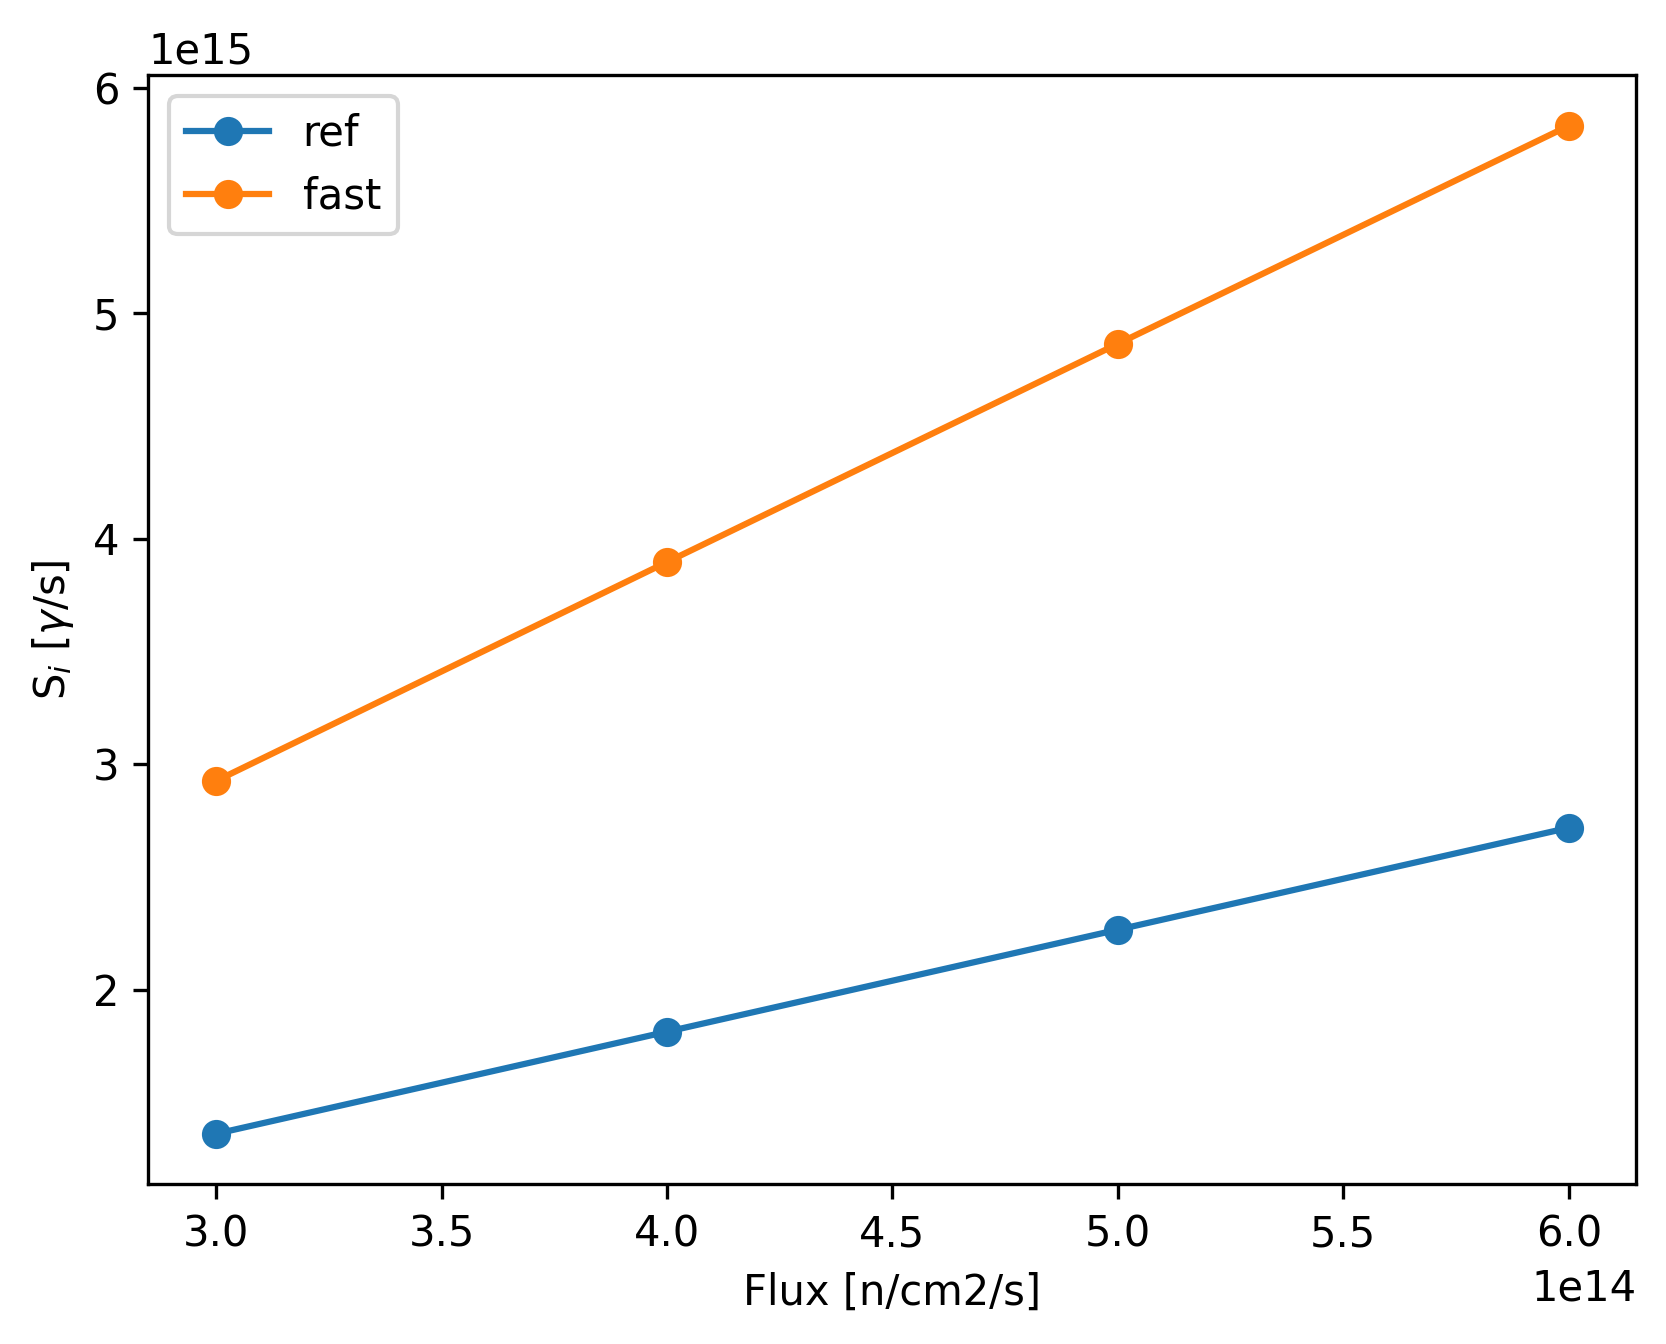
\includegraphics[width=0.7\textwidth]{figures/fast-res25_Si}
    \caption{Photon emission rate.}
  \end{subfigure}
  \hfill
  \caption{Sensitivity analysis for manganese.}
  \label{fig:sens-mn}
\end{figure}

\begin{figure}[htbp!] % or H
  \centering
  \begin{subfigure}[b]{0.49\textwidth}
    \centering
    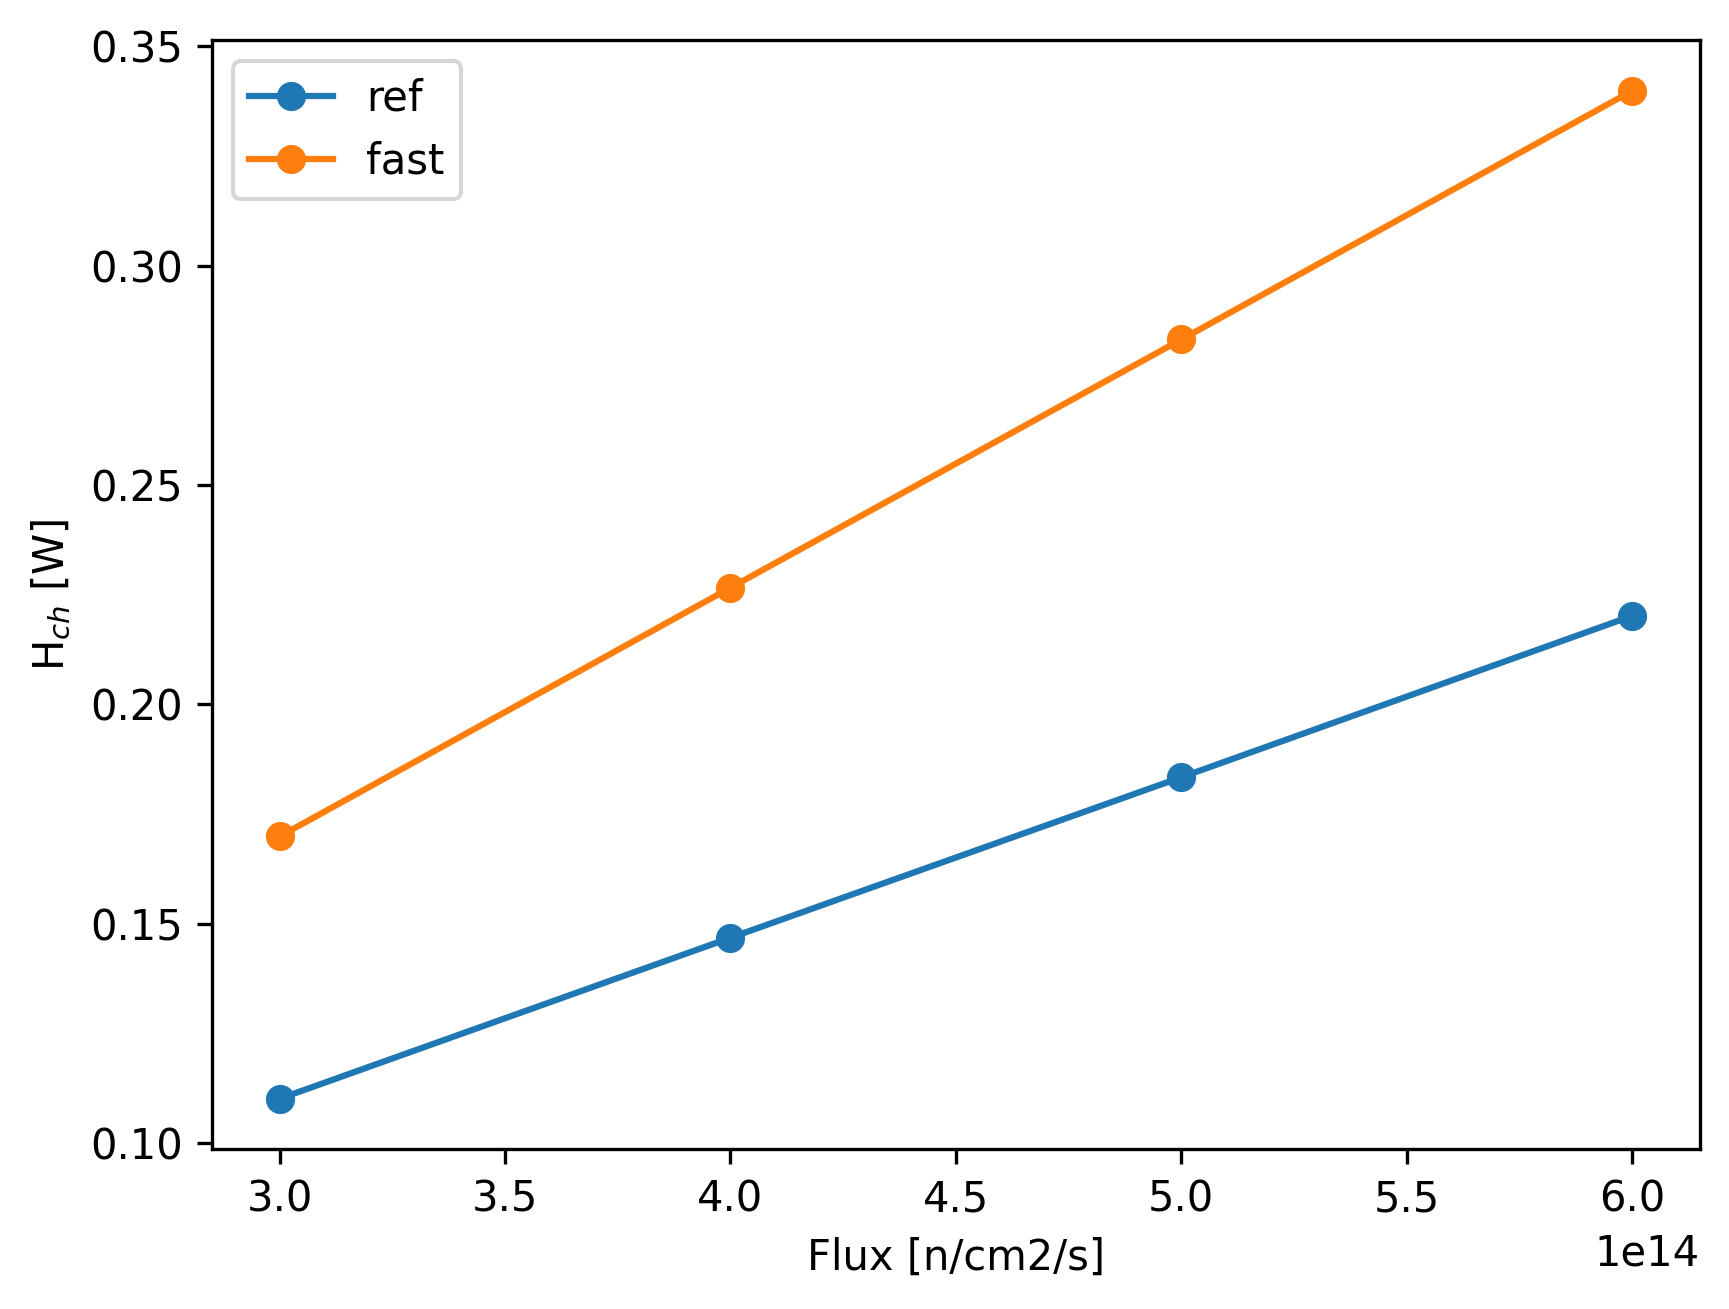
\includegraphics[width=0.7\textwidth]{figures/fast-res40_hch}
    \caption{Energy deposited by charged particles.}
  \end{subfigure}
  \hfill
  \begin{subfigure}[b]{0.49\textwidth}
    \centering
    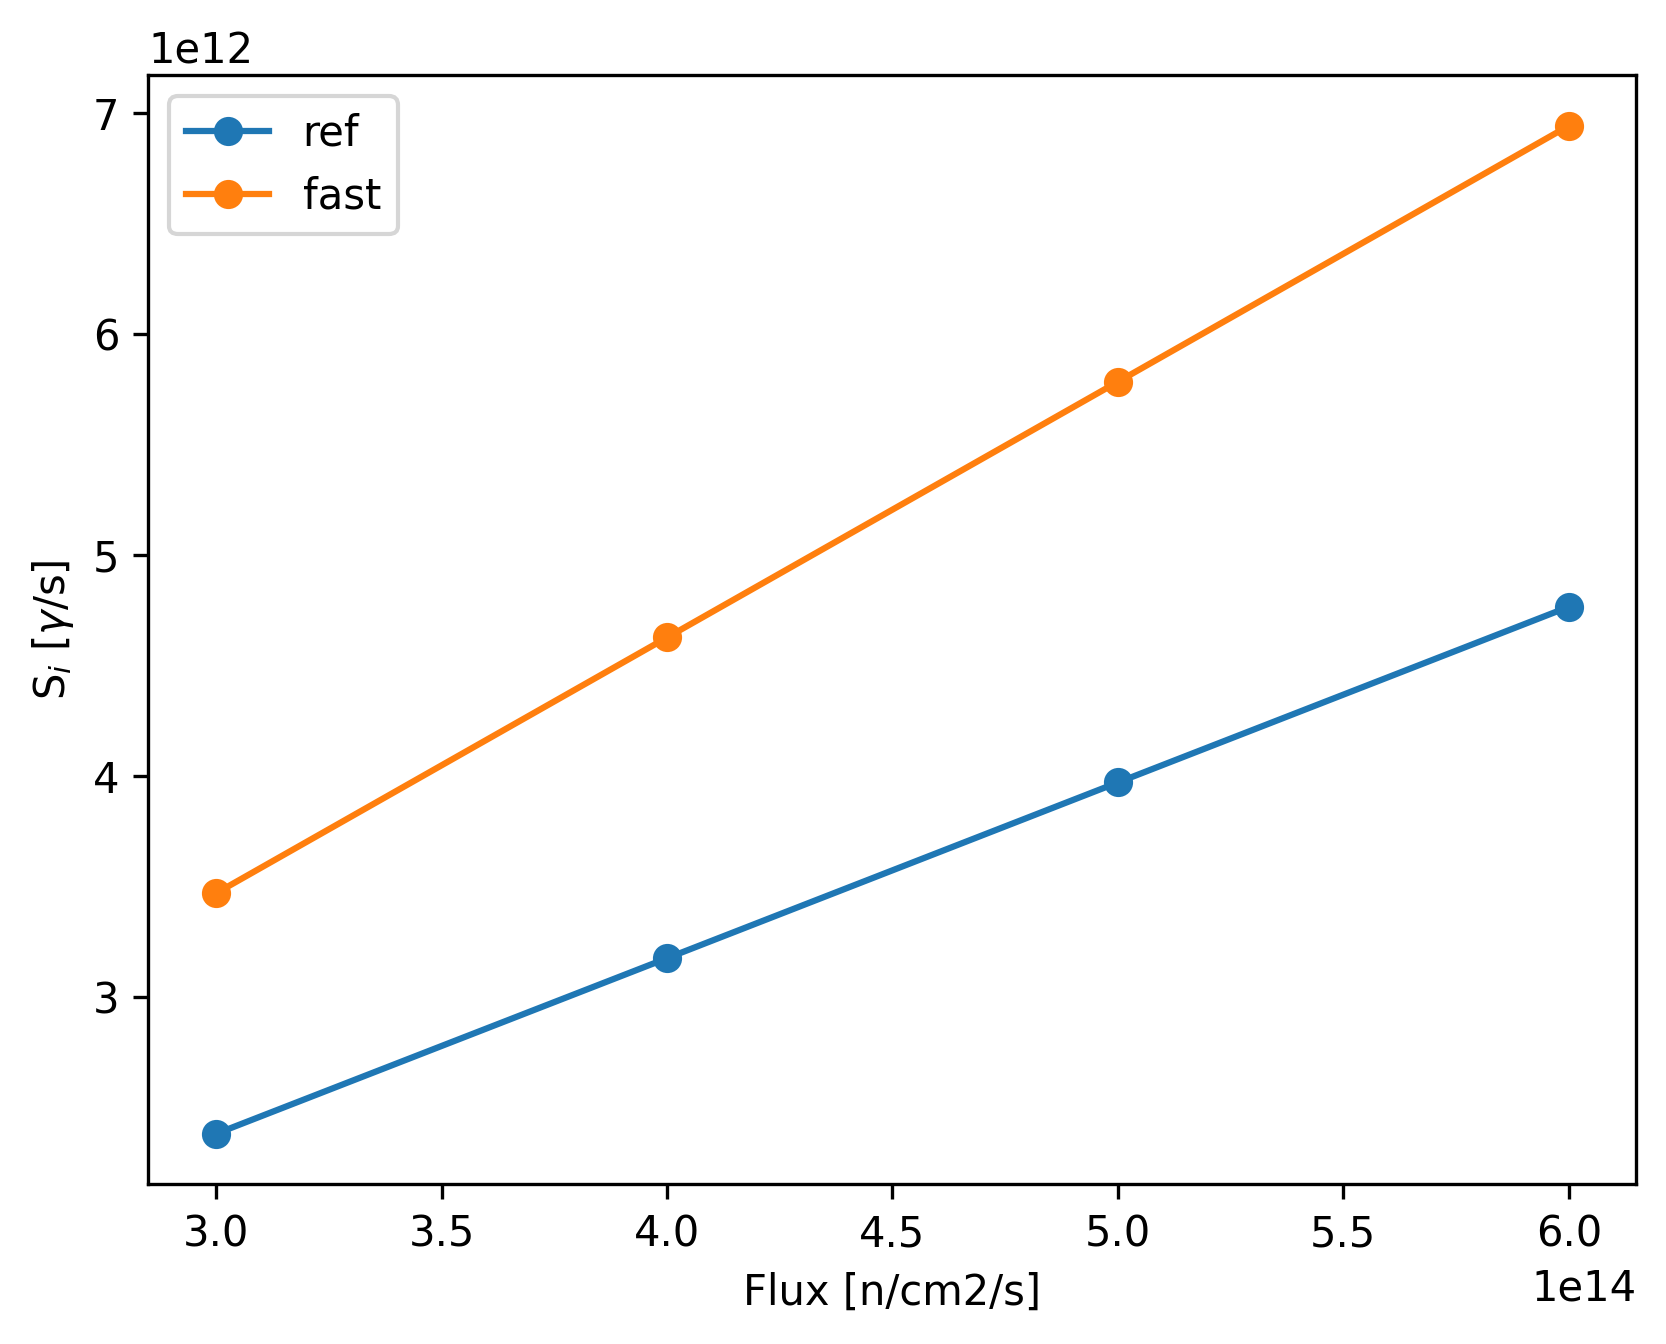
\includegraphics[width=0.7\textwidth]{figures/fast-res40_Si}
    \caption{Photon emission rate.}
  \end{subfigure}
  \hfill
  \caption{Sensitivity analysis for zirconium.}
  \label{fig:sens-zr}
\end{figure}

\begin{figure}[htbp!] % or H
  \centering
  \begin{subfigure}[b]{0.49\textwidth}
    \centering
    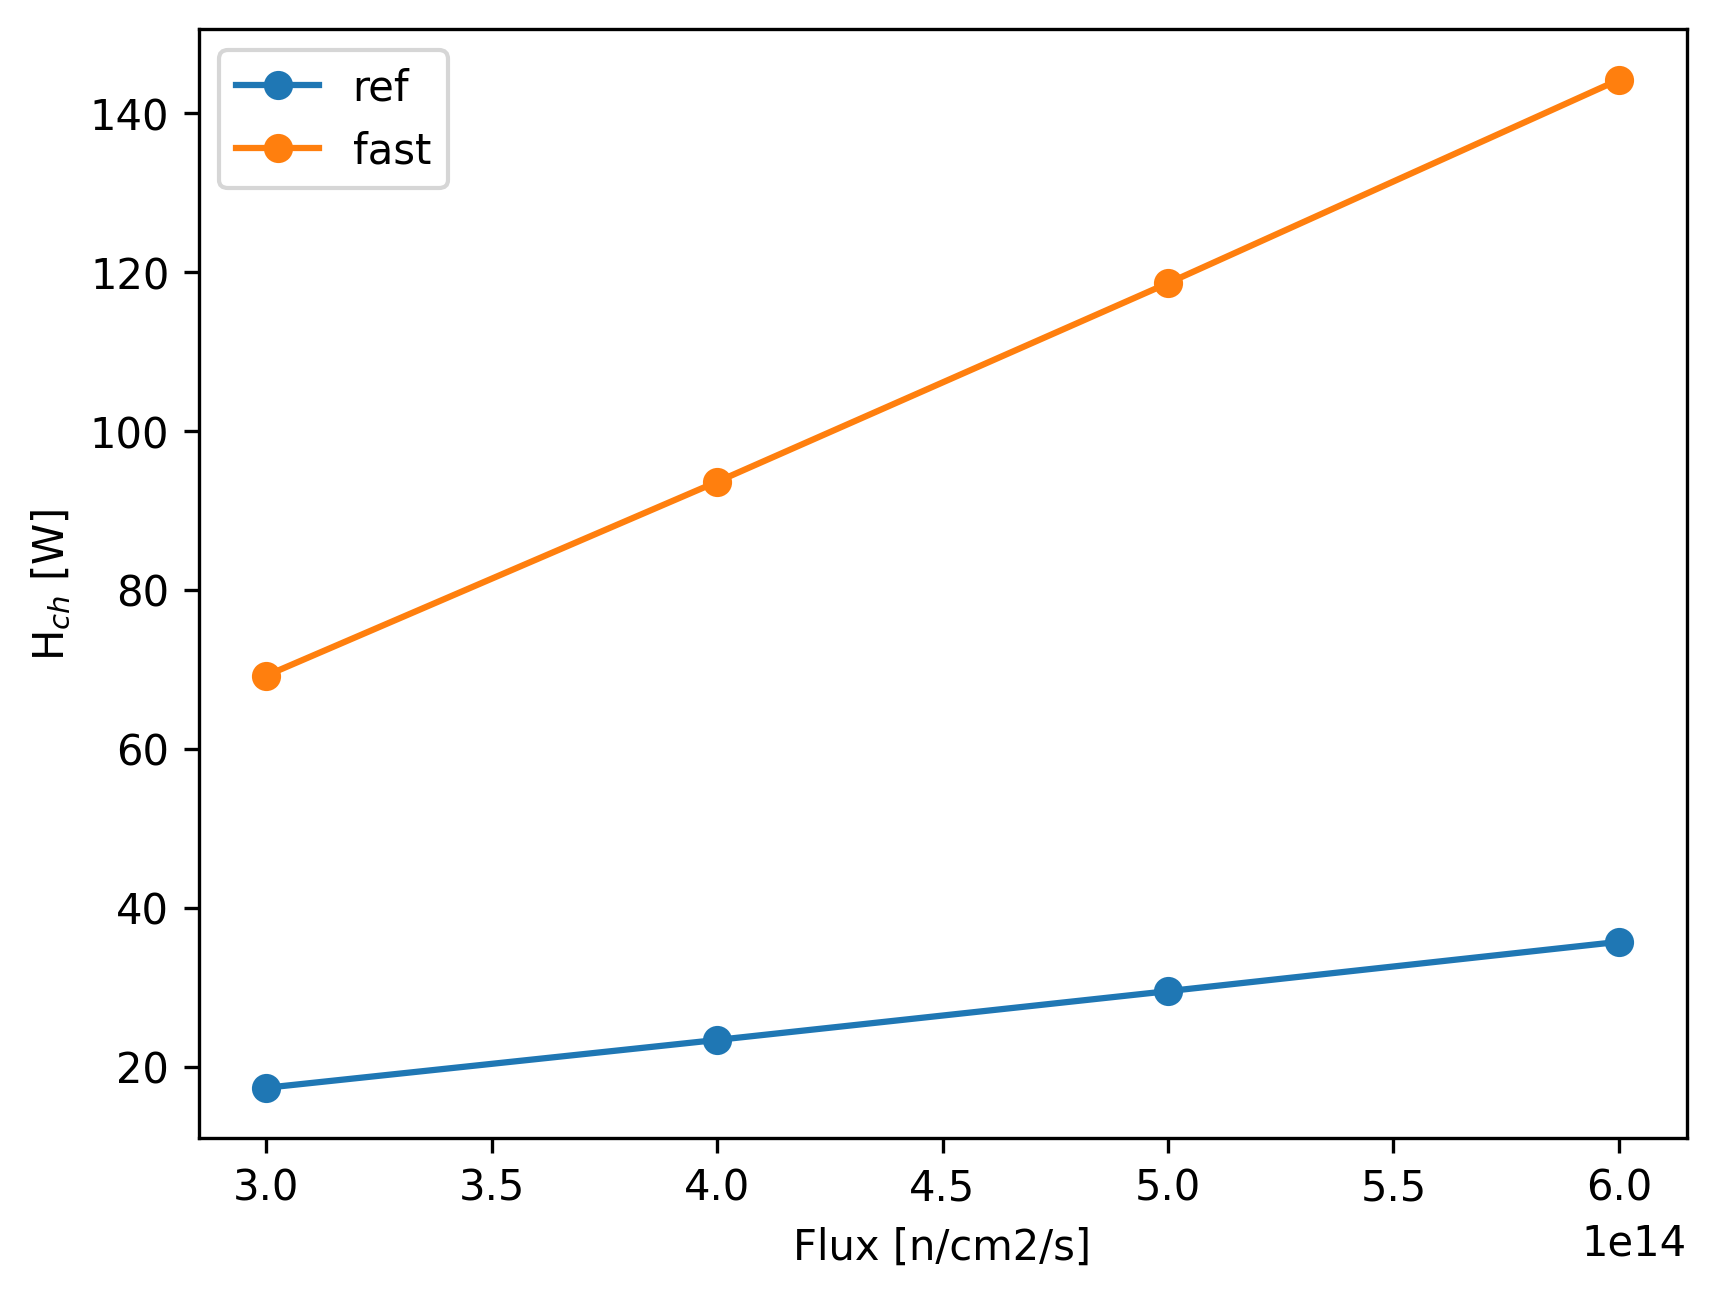
\includegraphics[width=0.7\textwidth]{figures/fast-res74_hch}
    \caption{Energy deposited by charged particles.}
  \end{subfigure}
  \hfill
  \begin{subfigure}[b]{0.49\textwidth}
    \centering
    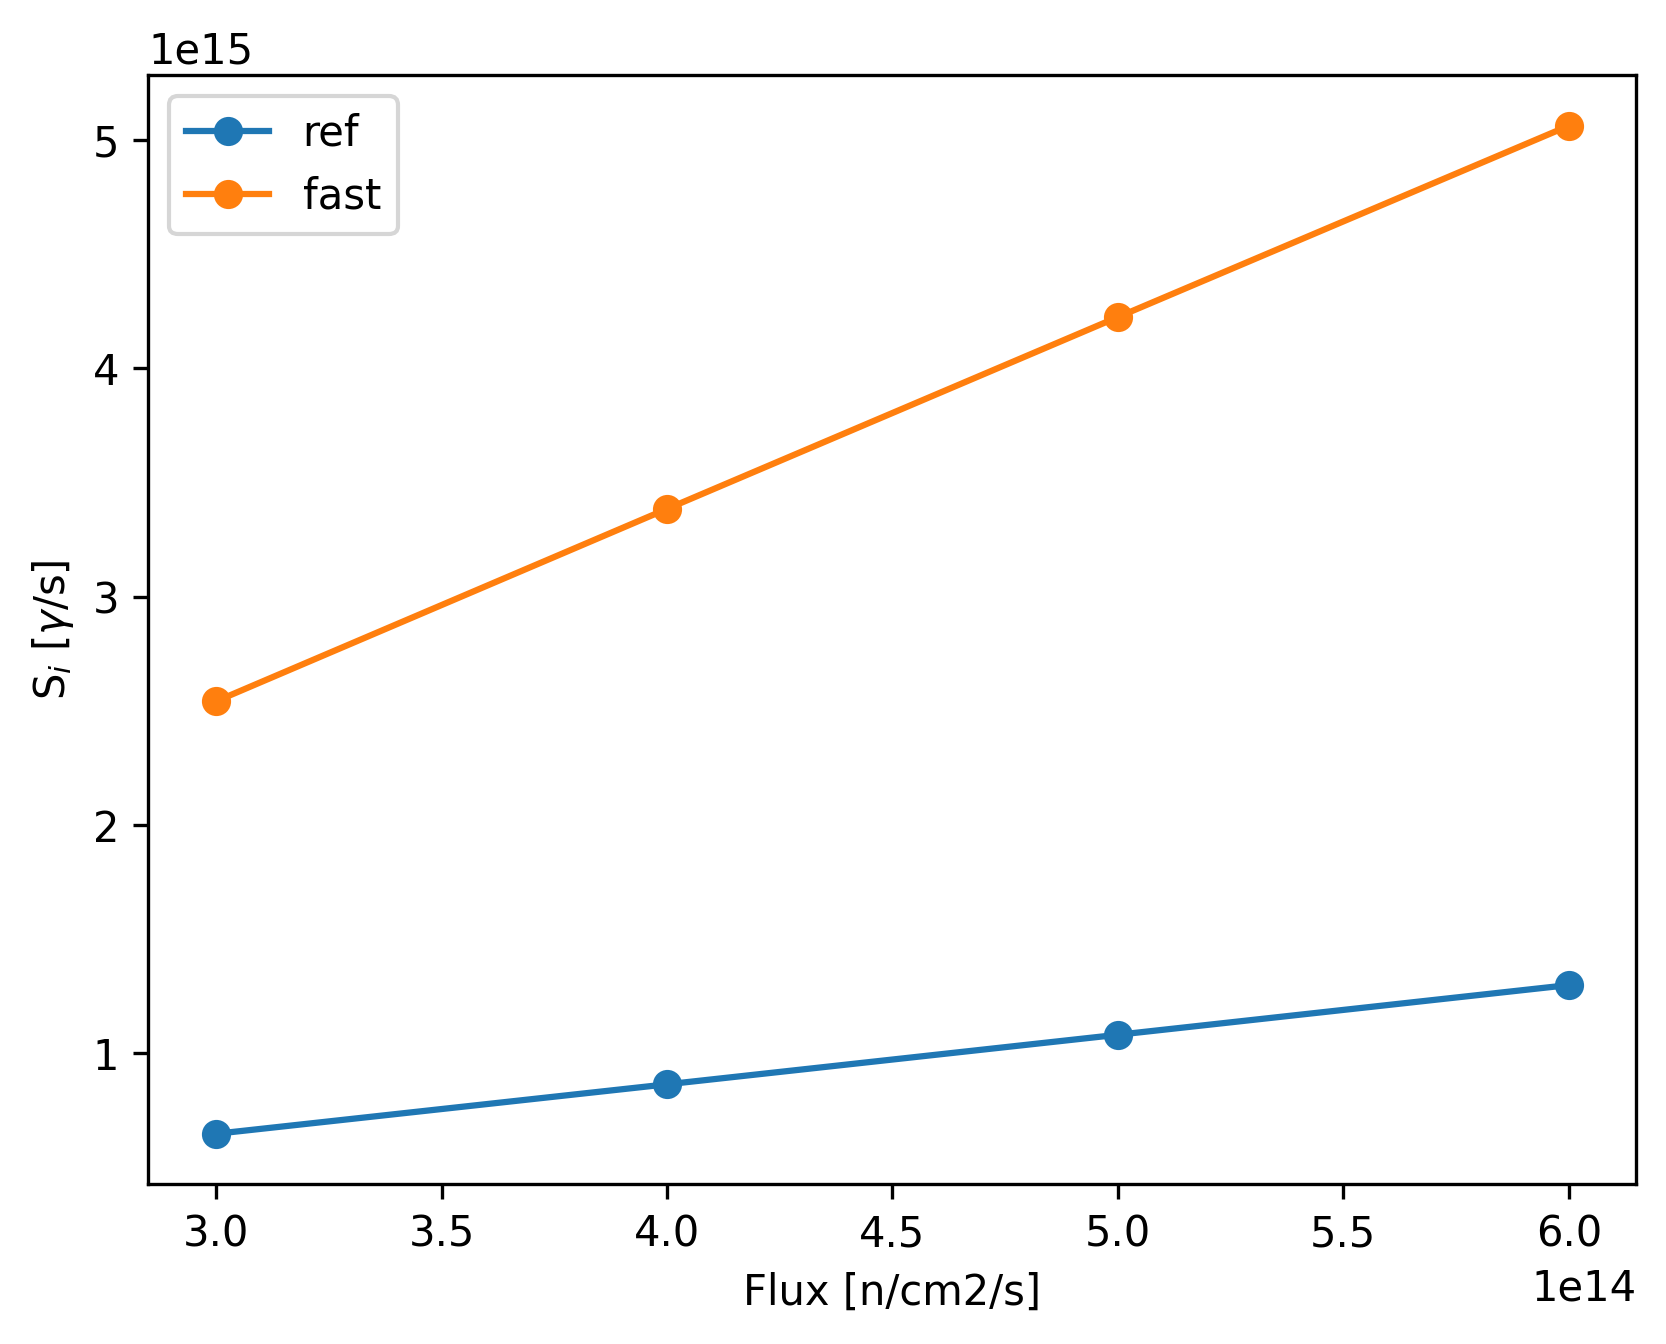
\includegraphics[width=0.7\textwidth]{figures/fast-res74_Si}
    \caption{Photon emission rate.}
  \end{subfigure}
  \hfill
  \caption{Sensitivity analysis for tungsten.}
  \label{fig:sens-w}
\end{figure}

\begin{figure}[htbp!] % or H
  \centering
  \begin{subfigure}[b]{0.49\textwidth}
    \centering
    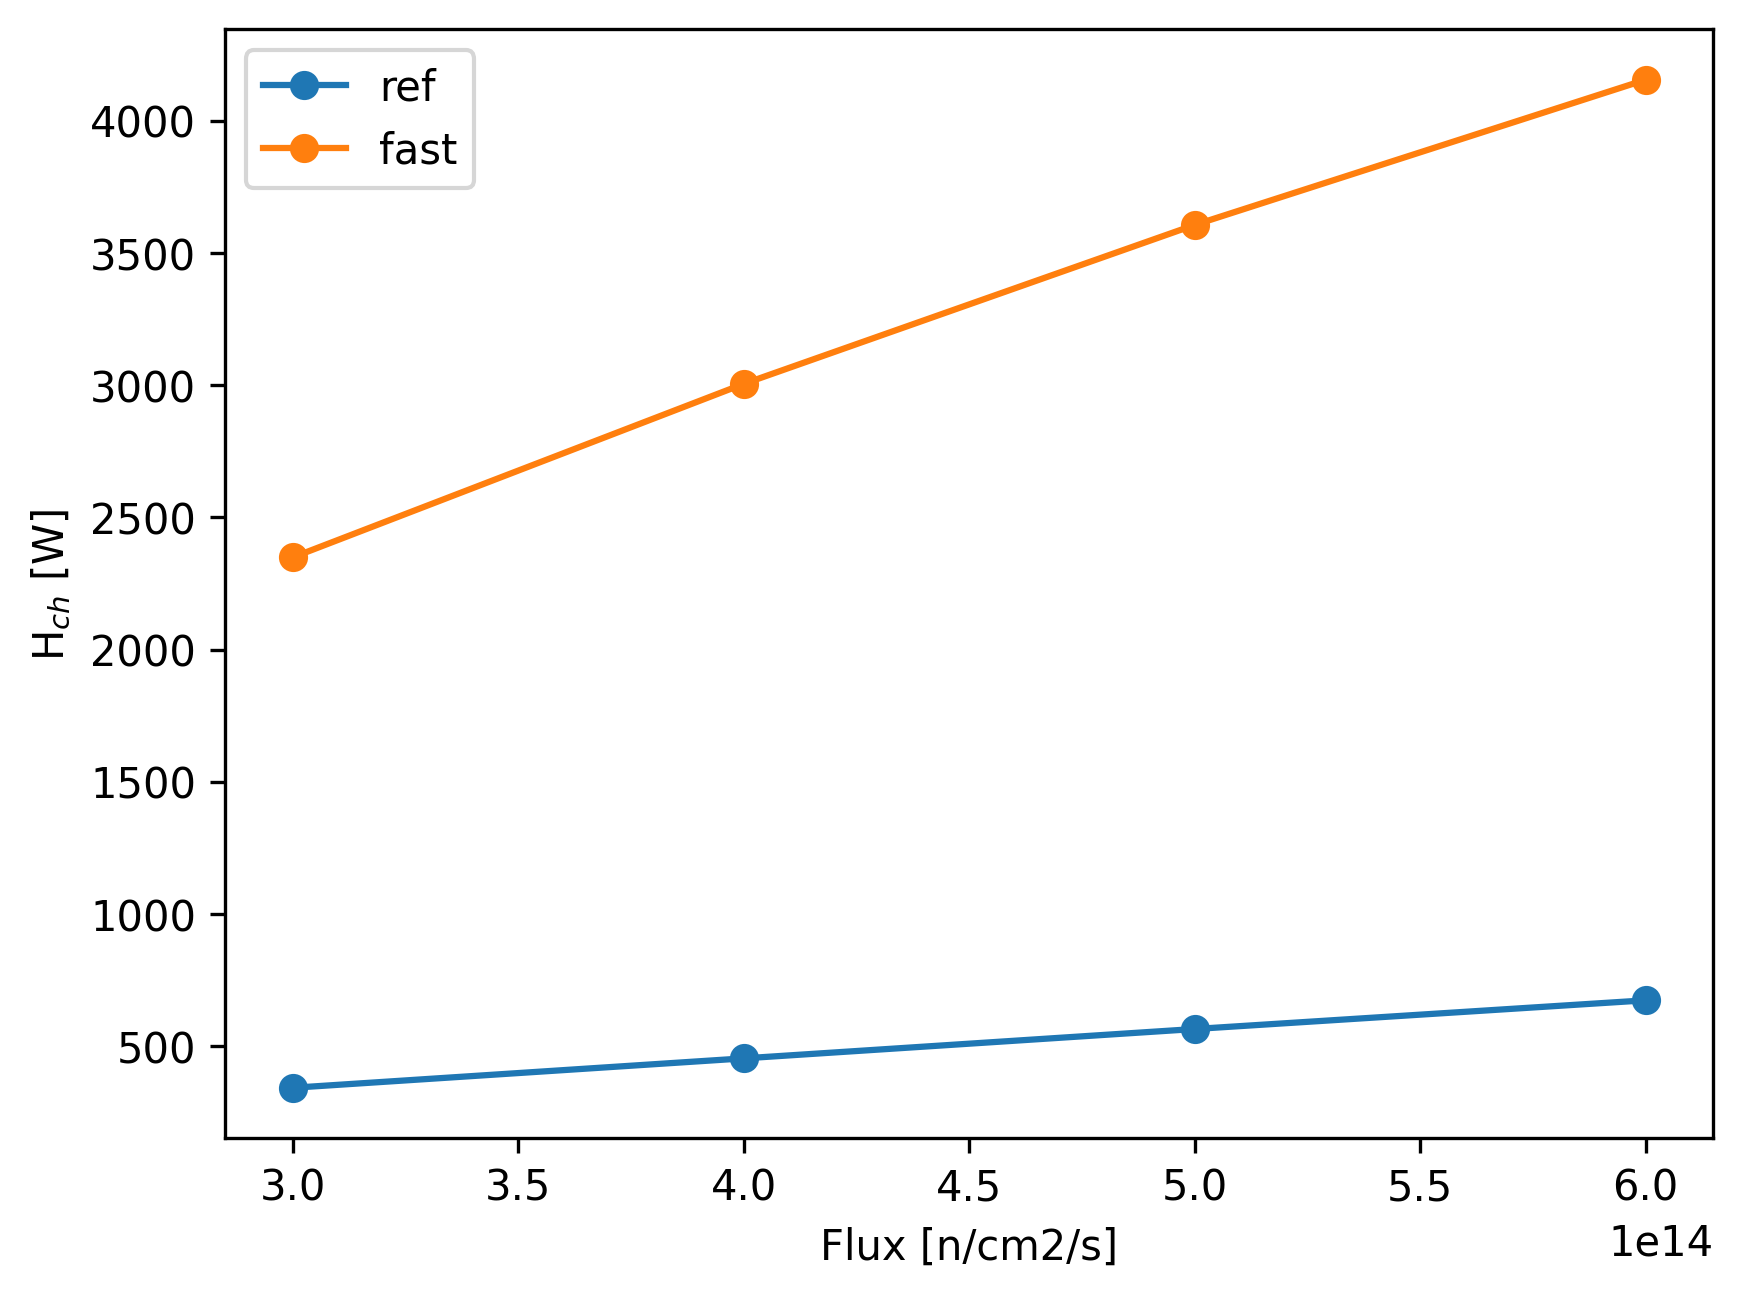
\includegraphics[width=0.7\textwidth]{figures/fast-res92_4_4_hch}
    \caption{Energy deposited by charged particles.}
  \end{subfigure}
  \hfill
  \begin{subfigure}[b]{0.49\textwidth}
    \centering
    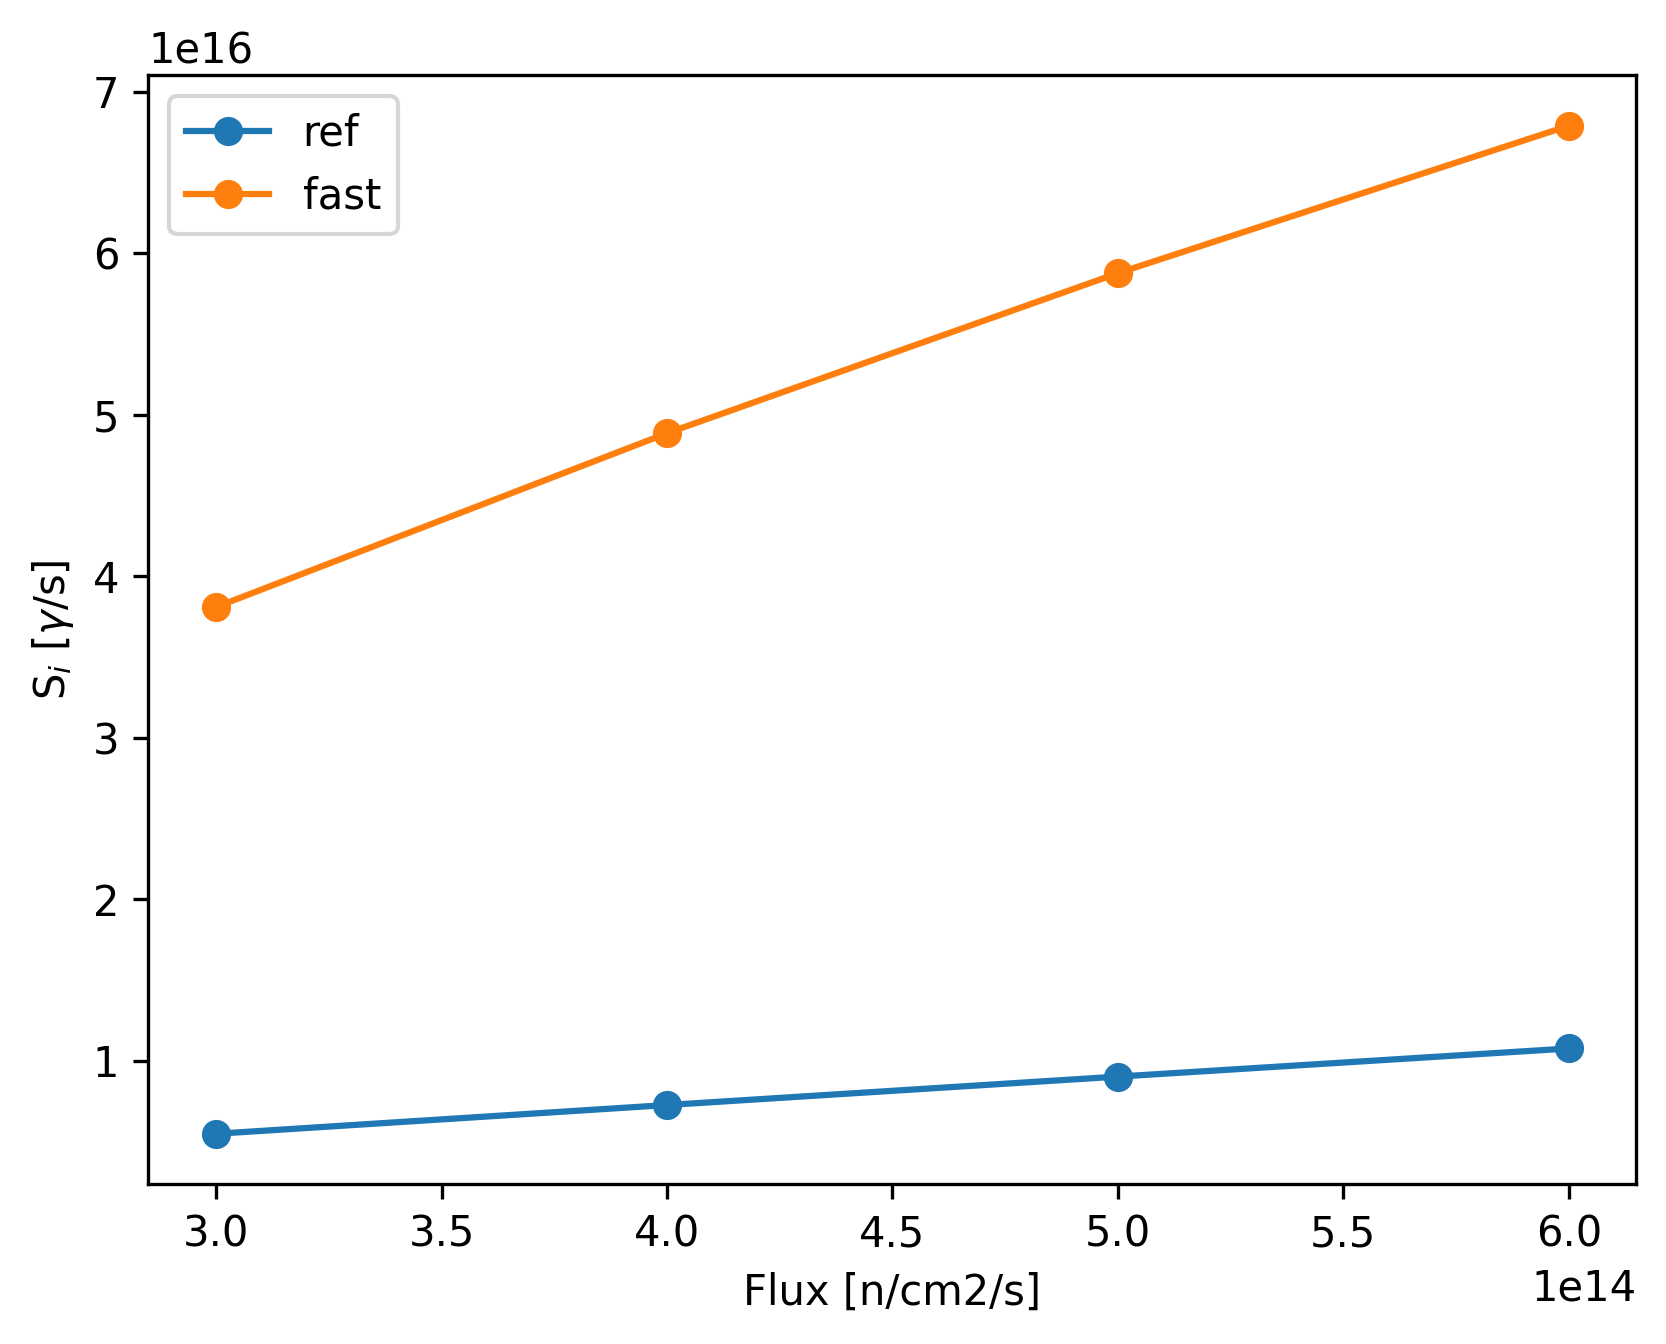
\includegraphics[width=0.7\textwidth]{figures/fast-res92_4_4_Si}
    \caption{Photon emission rate.}
  \end{subfigure}
  \hfill
  \caption{Sensitivity analysis for 20\%-enriched uranium.}
  \label{fig:sens-u}
\end{figure}

% Results
Table \ref{tab:fast-calc} compares the results using the fast calculation and the reference results obtained using the delayed heating calculation workflow.
The fast calculation method overestimates the delayed heating.
And while for some materials, such as aluminum and zirconium, the overestimation is minimal, for other materials, such as manganese, tungsten, and uranium, the overestimation is considerably larger.
The last step in the comparison is the delayed heating over time, shown in Figures \ref{fig:time-1} to \ref{fig:time-3}.
The delayed heating results confirm the observations in the sensitivity analysis, shown above.
The fast calculation yields accurate results for aluminum and zirconium, while it overestimates the delayed heating in experiments of manganese, tungsten, and uranium.

% Table
\begin{table}[htbp!]
  \centering
  \caption{Comparison of total heat deposited in experiments of selected materials for the fast calculation and the reference results of the delayed heating calculation workflow.}
  \label{tab:fast-calc}
  \begin{tabular}{ccccc}
    \toprule
    Material     & Atomic Number  & Fast [W]   & Reference [W]   & Rel. Diff. [\%] \\
    \midrule
    Aluminum     & 13             & 18.35      & 18.20           & 0.87            \\
    Manganese    & 25             & 375.1      & 169.37          & 121.49          \\
    Zirconium    & 40             & 38.36      & 38.24           & 0.31            \\
    Tungsten     & 74             & 356.19     & 164.46          & 116.58          \\
    Uranium ($\varepsilon$ = 20\%) & 92  & 5880.80  & 994.52     & 491.31          \\
    \bottomrule
  \end{tabular}
\end{table}

\begin{figure}[htbp!] % or H
  \centering
  \begin{subfigure}[b]{0.49\textwidth}
    \centering
    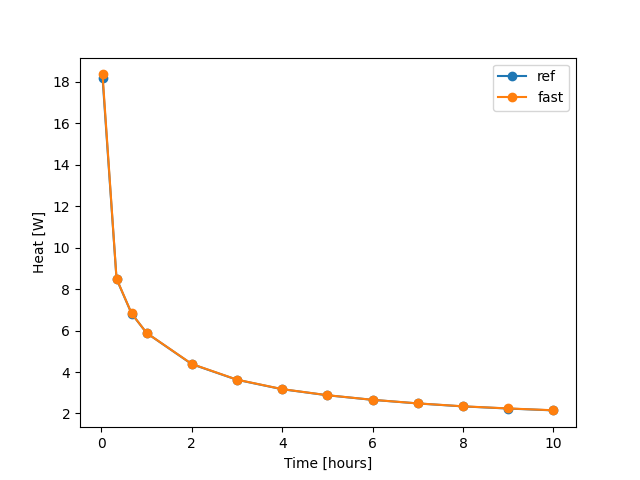
\includegraphics[width=0.7\textwidth]{figures/fast-13_overtime}
    \caption{Aluminum.}
  \end{subfigure}
  \hfill
  \begin{subfigure}[b]{0.49\textwidth}
    \centering
    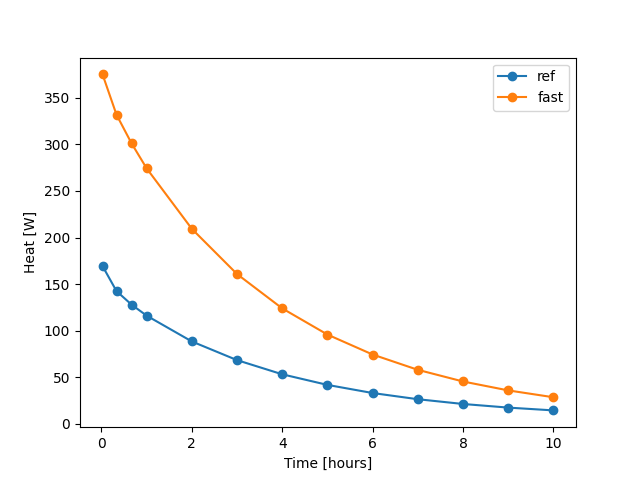
\includegraphics[width=0.7\textwidth]{figures/fast-25_overtime}
    \caption{Manganese.}
  \end{subfigure}
  \hfill
  \caption{Comparison of the delayed heating over time for the reference workflow and the fast calculation for experiments of selected materials.}
  \label{fig:time-1}
\end{figure}

\begin{figure}[htbp!] % or H
  \centering
  \begin{subfigure}[b]{0.49\textwidth}
    \centering
    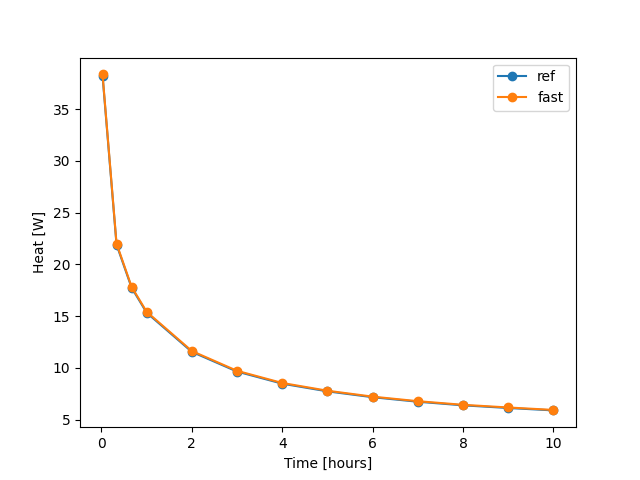
\includegraphics[width=0.7\textwidth]{figures/fast-40_overtime}
    \caption{Zirconium.}
  \end{subfigure}
  \hfill
  \begin{subfigure}[b]{0.49\textwidth}
    \centering
    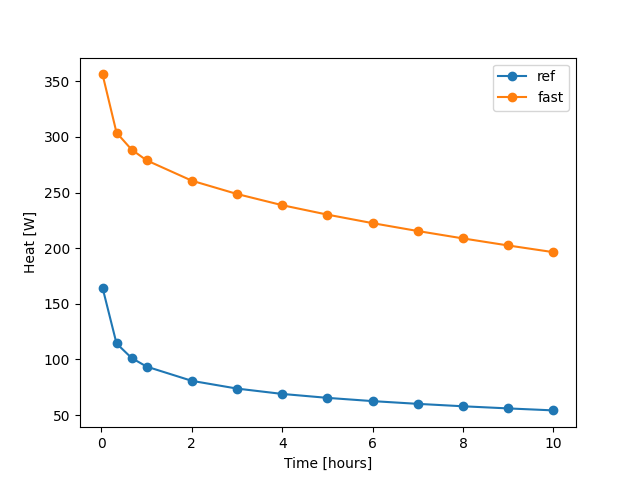
\includegraphics[width=0.7\textwidth]{figures/fast-74_overtime}
    \caption{Tungsten.}
  \end{subfigure}
  \hfill
  \caption{Comparison of the delayed heating over time for the reference workflow and the fast calculation for experiments of selected materials.}
  \label{fig:time-2}
\end{figure}

\begin{figure}[htbp!]
  \begin{center}
    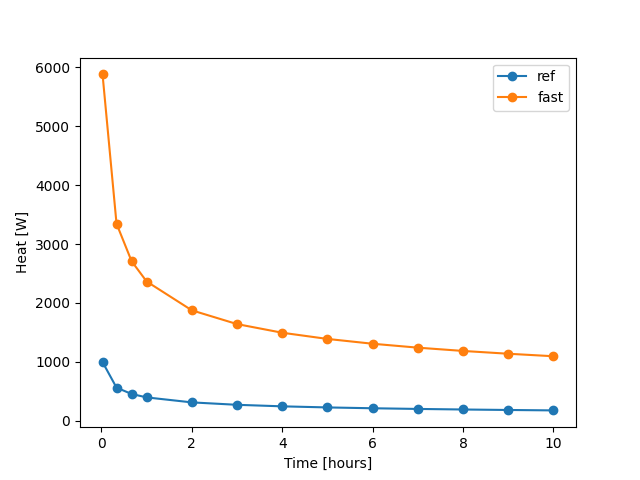
\includegraphics[width=0.42\linewidth]{figures/fast-92_4_4_overtime}
  \end{center}
  \caption{Comparison of the delayed heating over time for the reference workflow and the fast calculation for an experiment of 20\%-enriched uranium.}
  \label{fig:time-3}
\end{figure}

% Conclusion
These results show that the fast calculation is accurate for some cases and excessively conservative for others.
While a conservative approach may be desirable for some cases, this thesis investigates more accurate calculation methods.
Consequently, this section shows that the fast calculation is not suitable for this work's objectives, concluding that the neutron-transport simulations cannot be avoided.
The next section introduces a different approach and investigates its suitability.


\section{Generic Material Irradiation Database}
\label{sec:irradatabase}

% Intro to method
This section proposes the creation of a generic material irradiation database to decrease the burden of the delayed heating calculation in research reactor experiments.
The database is created by utilizing the calculation workflow defined in Chapter \ref{ch:delayedheat} repeatedly to obtain the delayed heating in experiments composed of pure chemical elements.
Nevertheless, an experiment is usually made of a mix of materials.
Hence, this work establishes a method using the database to calculate the delayed heating in experiments of arbitrary material composition.
This method enables the delayed heating calculation based on pre-computed values instead of re-doing the calculations.

% The following formula calculates the delayed heating in an experiment composed of several materials
% \begin{align}
% H_{j,M} &= \mathlarger{\sum}_i H_{j,i}(\rho_i)  \label{eq:data-1} \\
% H_{j,i}(\rho_i) &= \rho_i f(\rho_i)  \label{eq:data-2} \\
% f_{non-fiss}(\rho_i) &= H_{j,i}^o / \rho_i^o  \label{eq:data-3} \\
% f_{fiss}(\rho_i) &= H_{j,i}^k / \rho_i^k  \label{eq:data-4}
% \end{align}
% where $H_{j, M}$ is the heating component $j$ of the mix and $\rho$ is the density.
% The heating component $j$ could be either the charged particles, transported gammas, or total contributions.
% $H_{j,i}$ and $\rho_i$ correspond to the heating values and density of material $i$ in the mix.
% The formula contemplates two cases, fissile and non-fissile materials.
% The calculation of $H_{j,i}(\rho_i)$ requires a functional form for $f(\rho_i)$, being constant for non-fissile (Eq. \ref{eq:data-3}) and density-dependent for fissile materials (Eq. \ref{eq:data-4}).
% $H_{j,i}^o$ corresponds to the heating values for an experiment made of material $i$ only with a density value equal to its theoretical density $\rho_i^o$.
% $H_{j,i}^k$ corresponds to the heating values for an experiment made of material $i$ only with a density value equal to $\rho_i^k$.
% As $f_{fiss}$ is density-dependent, it requires multiple samples of $H_{i,j}^k/\rho_i^k$ for interpolating between adjacent values.

The following formula calculates the delayed heating in an experiment composed of several materials
\begin{align}
H_{j,M} &= \mathlarger{\sum}_i H_{j,i}(m_i)  \label{eq:data-1} \\
H_{j,i}(m_i) &= m_i f(m_i)  \label{eq:data-2} \\
f_{non-fiss}(m_i) &= H_{j,i}^o / m_i^o  \label{eq:data-3} \\
f_{fiss}(m_i) &= H_{j,i}^k / m_i^k  \label{eq:data-4}
\end{align}
where $H_{j, M}$ is the heating component $j$ of the mix, which could be either the charged particles, transported gammas, or total contributions.
$H_{j,i}$ and $m_i$ correspond to the heating values and mass of material $i$ in the mix.
The formula contemplates two cases: fissile and non-fissile materials.
The calculation of $H_{j,i}(m_i)$ requires a functional form for $f(m_i)$, being constant for non-fissile (Equation \ref{eq:data-3}) and mass-dependent for fissile materials (Equation \ref{eq:data-4}).
$H_{j,i}^o$ corresponds to the heating values for an experiment made of material $i$ and mass $m_i^o$, which is the mass of an experiment with density equal to the material's theoretical density $\rho_i^o$.
$H_{j,i}^k$ corresponds to the heating values for an experiment made of material $i$ and mass $m_i^k$, which is an arbitrary value.
As $f_{fiss}$ is mass-dependent, it requires multiple samples of $H_{i,j}^k/m_i^k$ for interpolating between adjacent values.

Because the Equations \ref{eq:data-2} to \ref{eq:data-4} consider a mass ratio, when the volume of the database and the experiment is the same, the mass ratio can be simplified into a density ratio.
The following exercises consider this case, and the calculations are based on the experiment density instead of experiment mass.

% TODO: Need to talk about the combination of fissile material. What results to show ?


\subsection{Demonstration exercise}

The exercise configuration and dimensions can be found in Section \ref{sec:demo}.
The experiment is irradiated for a period of 50 days with the reactor operating at a constant power of 5 MWth.
After that period, the reactor shuts down, and the heat deposited in the experiment is calculated immediately after shutdown.
To avoid the prompt-gamma contributions (emitted within 5 $\times$ 10$^{-8}$ seconds \cite{ilas_impact_2013}), the first step is taken 1 second after shutdown.
The reactor regions considered contributing to the experiment heating are the fuel elements and the experiment itself, while the activation of the moderator is neglected.

% Results from 14-
% Bronze
The following analyses focus on the delayed heating calculation for a mix of materials.
The first analysis considers an experiment of an arbitrary alloy: bronze, which is an alloy of copper and tin.
Bronze has a density of 8.73 g/cm$^3$, and the weight fractions are 88\% and 12\% for copper and tin, respectively.
Table \ref{tab:demo-brz} summarizes the results for the energy deposited by charged particles ($H_{ch}$), energy deposited by photon transport ($H_{\gamma, Tr}$), and total heat deposited ($H_{T}$).
The results from the generic material irradiation database method are based on the delayed heating of samples of pure copper (8.96 g/cm$^3$) and pure tin (5.75 g/cm$^3$).
The calculated values coincide with the reference values.
The relative difference for $H_{ch}$ is the largest, but it is still smaller than 5\%.

\begin{table}[htbp!]
  \centering
  \caption{Comparison of delayed heating for the generic material irradiation database method and reference calculation for an experiment of bronze.}
  \label{tab:demo-brz}
  \begin{tabular}{cccc}
    \toprule
                    & \multicolumn{1}{c}{\begin{tabular}[c]{@{}c@{}}Irradiation  database\\method [W]\end{tabular}} & \multicolumn{1}{c}{\begin{tabular}[c]{@{}c@{}}Reference\\calculation [W]\end{tabular}} & Rel. Diff [\%] \\
    \midrule
    $H_{ch}$            & 15.54   & 16.24   & -4.31  \\
    $H_{\gamma, Tr}$    & 49.75   & 50.17   & -0.84  \\
    $H_{T}$             & 65.30   & 66.41   & -1.67  \\
    \bottomrule
  \end{tabular}
\end{table}

% Bronze, why it works
The following analysis demonstrates why a constant function representing $f_{non-fiss}$ yields a good approximation.
Figure \ref{fig:H_rho1} displays $H_{j,i}/\rho_i$ as a function of $\rho$ for experiments of copper and tin.
The densities considered for copper are 2.25, 4.5, 6.75, and 8.96 g/cm$^3$ and for tin 1.5, 3.0, 4.5, and 5.75 g/cm$^3$.
These values represent approximately 25, 50, 75, and 100\% of the theoretical density for each material.
$H_{ch}$ represents less than 30\% and less than 2\% of $H_T$ for all densities for copper and tin, respectively.
For copper, the slope formed between the first and last values are -24\%, -9\%, and -13\% for $H_{ch}$, $H_{\gamma, Tr}$, and $H_{T}$, respectively.
For tin, the slope formed between the first and last values are -14\%, -16\%, and -16\% for $H_{ch}$, $H_{\gamma, Tr}$, and $H_{T}$, respectively.
The methodology introduced in this paper considers $H_{j,i}/\rho_i$ to be constant for non-fissile materials, as described by Equation \ref{eq:data-3}.
Although these curves have negative slopes, their magnitudes are relatively small, and as shown in Table \ref{tab:demo-brz}, a constant function still yields satisfactory results.

% H/\rho for non-fissile material
\begin{figure}[htbp!] %or H 
    \centering
    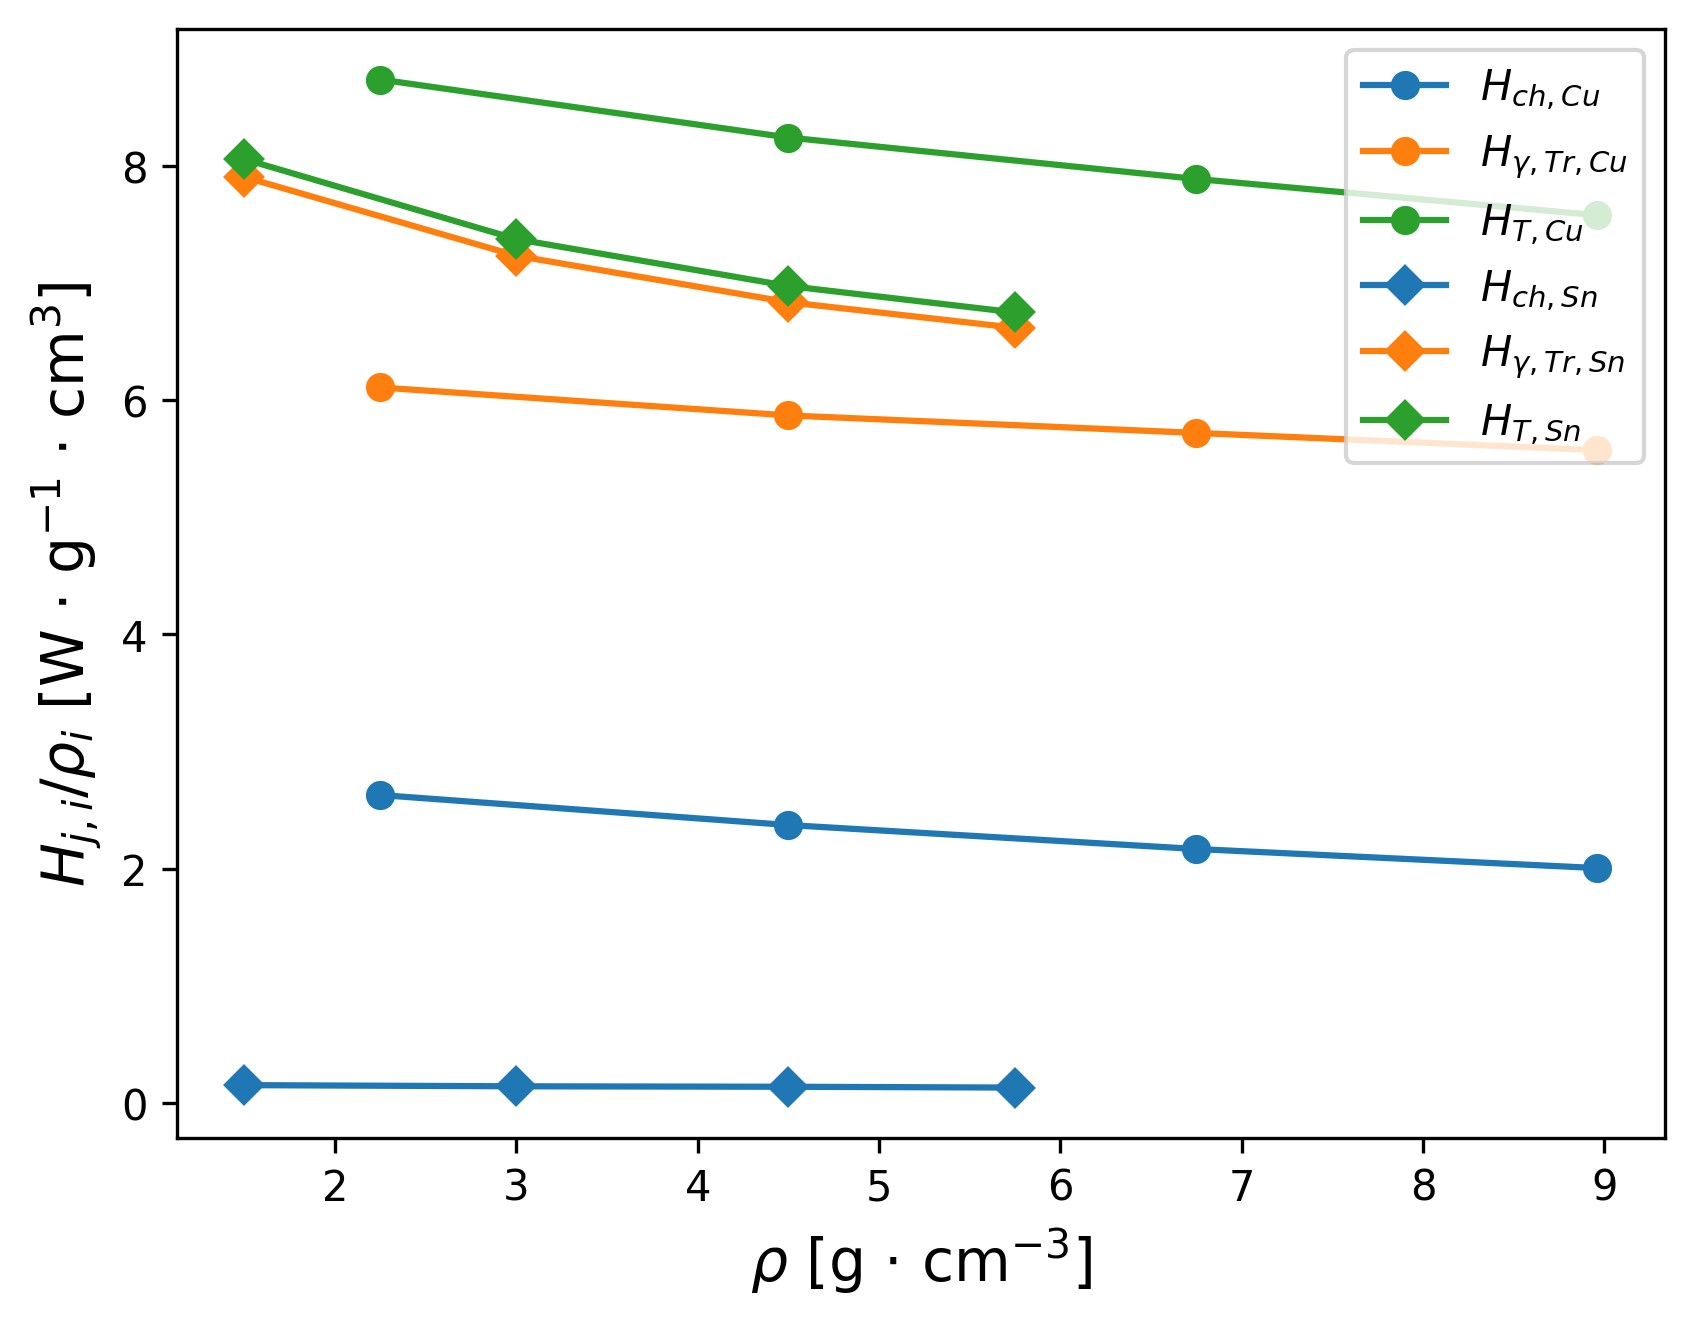
\includegraphics[width=0.55\linewidth]{figures/toy-Cu_Sn_rho}
    \hfill
    \caption{$H_{j}/\rho$ vs. $\rho$ for different experiment materials.}
    \label{fig:H_rho1}
\end{figure}

The following exercise considers an experiment including a fissile material, uranium nitride (UN).
This type of fuel has been extensively studied as one candidate accident tolerant fuel, due to its high thermal conductivity and high fissile element density \cite{un}.
Table \ref{tab:demo-un} summarizes the results for an experiment of UN.
The exercise adopts a 4\% enrichment for uranium.
The results from the generic material irradiation database correspond to the calculated value for uranium using a linear interpolation between database entries, while the contribution from nitrogen is considered negligible.
$H_T$ is calculated by adding together $H_{ch}$ and $H_{\gamma,Tr}$.
The relative difference of the results is less than 3\%, which confirms the choice of a linear interpolation to represent $f_{fiss}(\rho_i)$.

\begin{table}[htbp!]
  \centering
  \caption{Comparison of delayed heating for the generic material irradiation database method and reference calculation for an experiment of UN.}
  \label{tab:demo-un}
  \begin{tabular}{cccc}
    \toprule
                    & \multicolumn{1}{c}{\begin{tabular}[c]{@{}c@{}}Irradiation database\\method [W]\end{tabular}} & \multicolumn{1}{c}{\begin{tabular}[c]{@{}c@{}}Reference\\calculation [W]\end{tabular}} & Rel. Diff [\%] \\
    \midrule
    $H_{ch}$            & 273.1   & 267.0   &  2.3  \\
    $H_{\gamma, Tr}$    & 233.7   & 236.0   & -0.9  \\
    $H_{T}$             & 506.8   & 503.0   &  0.8  \\
    \bottomrule
  \end{tabular}
\end{table}

% UN, why it works
The following analysis demonstrates why the inclusion of a fissile material into the mix requires a linear interpolation between database entries to obtain $f_{fiss}$.
The exercise adopts the following uranium densities for the calculations: 1, 7, 13, and 19 g/cm$^3$.
The UN has a density of 13.5 g/cm$^3$, and the atomic fraction is 50\% for both elements.
Figure \ref{fig:H_rho2} displays $H_{j,i}/\rho_i$ as a function of $\rho$ for the experiment of uranium.
Only the values for the uranium are included because the delayed heating in a sample of pure nitrogen is negligible.
$H_{\gamma, Tr}/\rho$ is almost constant, while $H_{ch}/\rho$ decreases as the density increases.
% % Quadratic function R^2: 0.99
% % 0.07013153878082601 x^2 + -2.6293650151097636 x + 42.73063110509705

\begin{figure}[htbp!] %or H 
    \centering
    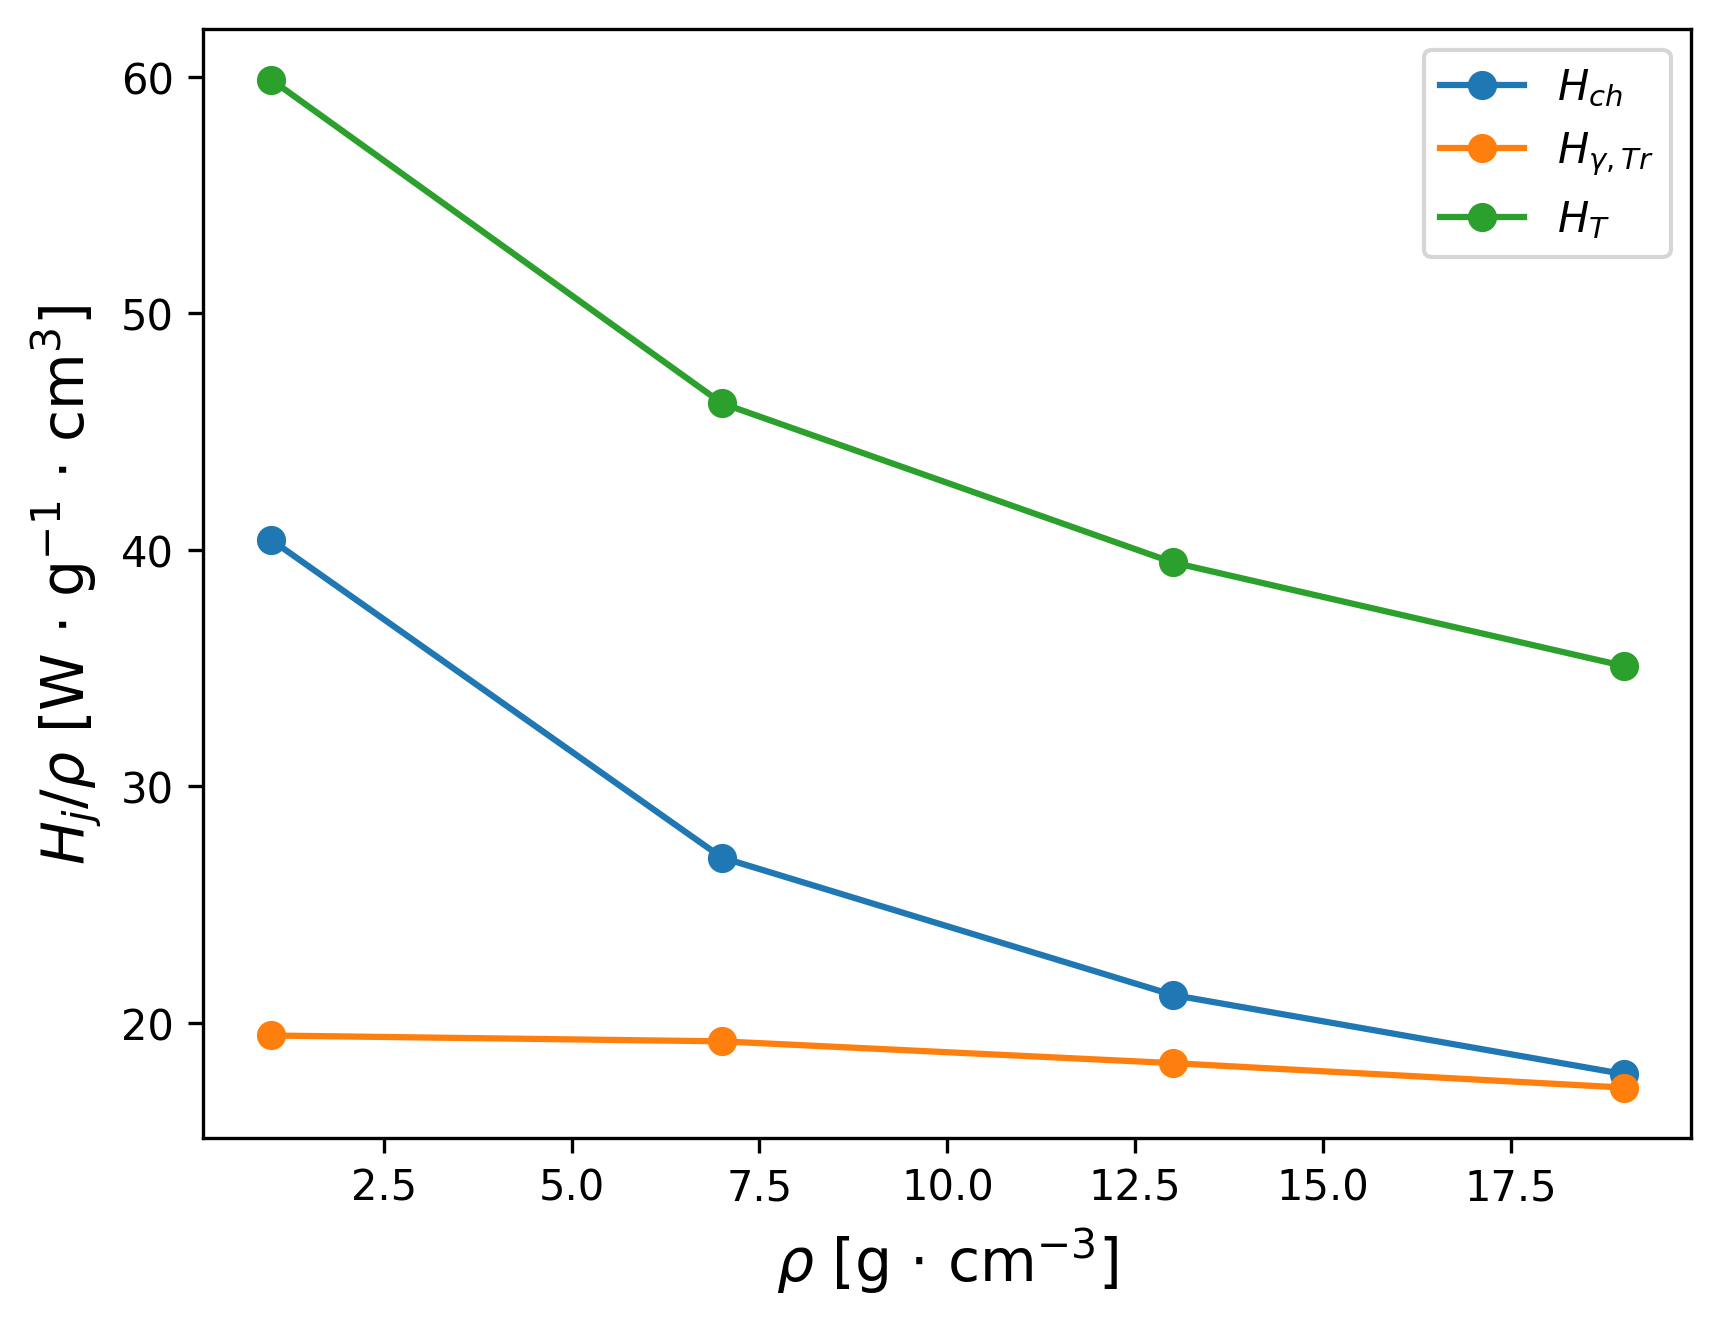
\includegraphics[width=0.55\linewidth]{figures/toy-U_rho}
    \hfill
    \caption{$H_{j}/\rho$ vs. $\rho$ for an experiment of 4\%-enriched uranium.}
    \label{fig:H_rho2}
\end{figure}

% Zirconium alloys
The following exercise considers three experiments of zirconium alloys: Zircaloy-2, Zircaloy-4, and ZrNb.
% Talk about the importance of these 3 alloys
Zirconium is a metal with excellent corrosion resistance, good mechanical properties, and very low thermal neutron cross-section \cite{zircaloy}.
Zircaloy-2 is composed of Zr-1.5Sn-0.15Fe-0.1Cr-0.05Ni and its primary use is as fuel cladding in \glspl*{BWR} and as calandria tubes in CANDU reactors.
Zircaloy-4 is composed of Zr-1.5Sn-0.2Fe-0.1Cr, which is a similar composition to Zircaloy-2 but removes the nickel and increases the iron weight for less hydrogen uptake, and it is used as fuel cladding in \gls*{PWR} and CANDU reactors.
ZrNb is composed of Zr-2.5Nb, wherein the niobium increases the alloy's strength, and it is used in pressure tubes in CANDU reactors.
%
Table \ref{tab:demo-zircaloy} displays the results for the three zirconium alloys.
The results from the generic material irradiation database method are based on the delayed heating of samples of pure zirconium (7.13 g/cm$^3$), pure tin (5.75 g/cm$^3$), pure iron (7.87 g/cm$^3$), pure chromium (7.18 g/cm$^3$), pure nickel (8.90 g/cm$^3$), and pure niobium (8.57 g/cm$^3$).
The reference calculation considers an experiment density of 6.56 g/cm$^3$, 6.56 g/cm$^3$, and 6.44 g/cm$^3$, for Zircaloy-2, Zircaloy-4, and ZrNb, respectively.
The calculated values show good agreement with respect to the reference values.
The relative difference for $H_{ch}$ is the largest for Zircaloy-2, while all the other relative differences are below 3\%.

\begin{table}[htbp!]
  \centering
  \caption{Comparison of delayed heating for the generic material irradiation database method and reference calculation for multiple experiments.}
  \label{tab:demo-zircaloy}
  \begin{tabular}{cccc}
    \toprule
                    & \multicolumn{1}{c}{\begin{tabular}[c]{@{}c@{}}Irradiation Database\\method [W]\end{tabular}} & \multicolumn{1}{c}{\begin{tabular}[c]{@{}c@{}}Reference\\calculation [W]\end{tabular}} & Rel. Diff [\%] \\
    \midrule
    \multicolumn{4}{c}{Zircaloy-2}                    \\
    \midrule
    $H_{ch}$            &  0.19   &  0.18   &  5.84   \\
    $H_{\gamma, Tr}$    & 38.42   & 38.39   &  0.07   \\
    $H_{T}$             & 38.61   & 38.57   &  0.10   \\
    \midrule
    \multicolumn{4}{c}{Zircaloy-4}                    \\
    \midrule
    $H_{ch}$            &  0.19   &  0.19   &  1.48   \\
    $H_{\gamma, Tr}$    & 38.42   & 38.40   &  0.06   \\
    $H_{T}$             & 38.61   & 38.58   &  0.06   \\
    \midrule
    \multicolumn{4}{c}{ZrNb}                          \\
    \midrule
    $H_{ch}$            &  0.19   &  0.19   &  2.49   \\
    $H_{\gamma, Tr}$    & 37.66   & 37.72   & -0.15   \\
    $H_{T}$             & 37.85   & 37.91   & -0.14   \\
    \midrule
    \multicolumn{4}{c}{U(nat)-Mo}                     \\
    \midrule
    $H_{ch}$            & 135.38   & 132.31  &  2.32  \\
    $H_{\gamma, Tr}$    & 196.06   & 191.66  &  2.30  \\
    $H_{T}$             & 331.44   & 323.97  &  2.31  \\
    \midrule
    \multicolumn{4}{c}{U(nat)-Nb}                     \\
    \midrule
    $H_{ch}$            & 129.13   & 127.35  &  1.39  \\
    $H_{\gamma, Tr}$    & 187.82   & 183.92  &  2.12  \\
    $H_{T}$             & 316.94   & 311.27  &  1.82  \\
    \midrule
    \multicolumn{4}{c}{U(20\%)3Si2Al}                 \\
    \midrule
    $H_{ch}$            & 254.96   & 247.48  &  3.02  \\
    $H_{\gamma, Tr}$    &  95.75   & 108.88  &-12.05  \\
    $H_{T}$             & 350.71   & 356.35  & -1.58  \\
    \midrule
    \multicolumn{4}{c}{Tungsten alloy}    \\
    \midrule
    $H_{ch}$            &  21.35   &  22.52  & -5.22  \\
    $H_{\gamma, Tr}$    & 129.20   & 132.33  & -2.37  \\
    $H_{T}$             & 150.54   & 154.85  & -2.78  \\
    \bottomrule
  \end{tabular}
\end{table}

% Uranium alloys
The following exercise considers three experiments containing uranium.
The first two are uranium-based alloys: U-9Mo and U-10Nb.
It is common for fissionable materials to exhibit anisotropic growth during neutron irradiation.
However, alloying uranium with elements such as molybdenum and niobium, causes the alloy to retain the metastable gamma phase during irradiation, and the anisotropic growth can be eliminated \cite{bleiberg_2004}.
% hutagaol_2022 - U3Si2Al
The third experiment is composed of U$_3$Si$_2$/Al, which is a typical material utilized in \gls*{MTR}-fuel plates.
% 
Table \ref{tab:demo-zircaloy} displays the results for the experiments containing uranium.

The calculations consider a natural uranium composition for the experiments of UMo and UNb and a 20\%-enriched uranium for the experiment of U$_3$Si$_2$/Al.
The results from the generic material irradiation database method are based on the delayed heating of samples of pure uranium, pure molybdenum, pure niobium, pure silicon, and pure aluminum.
The exercise adopts the following uranium densities for the calculations: 1, 7, 13, and 19 g/cm$^3$.
For molybdenum, niobium, silicon, and aluminum, the exercise uses densities of 10.22, 8.57, 2.33, and 2.70 g/cm$^3$, respectively.
The reference calculation considers an experiment density of 17.35, 16.51, and 5.76 g/cm$^3$, for UMo, UNb, and U$_3$Si$_2$/Al, respectively.
Most of the calculated values show good agreement with respect to the reference values, showing relative differences below 3\%, except $H_{ch}$ and $H_{\gamma, Tr}$ for U$_3$Si$_2$/Al.
The latter shows a relative difference of approximately 12\%, but as the charged particles have a larger contribution to the heating, the total heat is within 2\% of the reference value.

% Tungsten alloy
The following exercise considers an experiment of tungsten-nickel-iron alloy.
% 
Tungsten alloys are good candidates for fusion applications, due to tungsten's high melting point.
However, tungsten alone can be very brittle, and including small amounts of other metals, such as nickel and iron, creates a tougher alloy while retaining the high melting temperature \cite{wong_metals_2023}.
The alloy composition considered in this work is W-3.5Ni-1.5Fe.
%
Table \ref{tab:demo-zircaloy} displays the results for this alloy.
The calculated values show good agreement with respect to the reference values.
The largest relative difference is for $H_{ch}$, being around 5\%, while the rest of the relative differences are within 3\%.
% The largest contribution to the delayed heating comes from the gamma particles.

% % FeCrAl
% The following exercise considers two experiments of iron-chromium-aluminum (FeCrAl) alloys.
% % Talk about the importance of this alloy
% This type of alloy exhibits enhanced oxidation resistance in elevated temperature steam environments when compared to Zr-based alloys, making it a good cladding candidate for accident tolerant fuel in \glspl{LWR} \cite{field_accident_2017}.
% Additionally, it is stress corrosion cracking resistant and irradiation induced swelling resistant.
% The typical content ranges from 10 to 22\% for Cr, and from 4 to 8\% for Al.
% This exercise uses the following two compositions: Fe-22\%Cr-8\%Al and Fe-10\%Cr-4\%Al.

% %
% Table \ref{tab:demo-FeCrAl} displays the results for these two alloys.
% The results from the database method are based on the delayed heating of samples of pure Fe ($\rho_{Fe}$ = 7.87 g/cm$^3$), pure Cr ($\rho_{Cr}$ = 7.18 g/cm$^3$), and pure Al ($\rho_{Al}$ = 2.70 g/cm$^3$).
% The reference calculations consider an experiment density of 8 g/cm$^3$ for both alloys.
% The calculated values for $H_{\gamma, Tr}$ and $H_{T}$ show good agreement with respect to the reference values.
% The relative difference for $H_{ch}$ is the largest, being approximately 23\% for the first alloy.
% Because the material is not highly activated, this large relative difference does not affect the total heat deposition, having a relative difference below 1\%.

% \begin{table}[htbp!]
%   \centering
%   \caption{.}
%   \label{tab:demo-FeCrAl}
%   \begin{tabular}{cccc}
%     \toprule
%                     & \multicolumn{1}{c}{\begin{tabular}[c]{@{}c@{}}Database\\method [W]\end{tabular}} & \multicolumn{1}{c}{\begin{tabular}[c]{@{}c@{}}Reference\\calculation [W]\end{tabular}} & Rel. Diff [\%] \\
%     \midrule
%     \multicolumn{4}{c}{70\% Fe, 22\% Cr, 8\% Al}      \\
%     $H_{ch}$            &  0.82   &  0.67   & 22.77   \\
%     $H_{\gamma, Tr}$    & 42.23   & 42.00   &  0.56   \\
%     $H_{T}$             & 43.06   & 42.67   &  0.91   \\
%     \multicolumn{4}{c}{86\% Fe, 10\% Cr, 4\% Al}      \\
%     $H_{ch}$            &  0.43   &  0.35   & 21.24   \\
%     $H_{\gamma, Tr}$    & 42.20   & 42.09   &  0.27   \\
%     $H_{T}$             & 42.63   & 42.45   &  0.44   \\
%     \bottomrule
%   \end{tabular}
% \end{table}

% % RAFM
% The following exercise considers an experiment of reduced activation ferritic-martensitic (RAFM) steel, which is a promising material for fusion reactor structural applications due to its properties such as a reduced activation and elastic and thermal properties that do not differ from Grade91 steel, commonly used in power plants because of its low thermal expansion coefficient and high thermal conductivity \cite{tanigawa_2017}.
% This works considers the following composition Fe-9\%Cr–1\%W–0.2\%V–0.1\%Ta for the steel.

% % results
% Table \ref{tab:demo-RAFM} displays the results for this alloy.
% The results from the database method are based on the delayed heating of samples of pure Fe ($\rho_{Fe}$ = 7.87 g/cm$^3$), pure Cr ($\rho_{Cr}$ = 7.18 g/cm$^3$), pure W ($\rho_{W}$ = 19.3 g/cm$^3$), pure V ($\rho_{V}$ = 6.11 g/cm$^3$), and pure Ta ($\rho_{Ta}$ = 16.654 g/cm$^3$).
% The reference calculations consider an experiment density of 7.80 g/cm$^3$ for the alloy.
% The calculated values for $H_{\gamma, Tr}$ and $H_{T}$ show good agreement with respect to the reference values.
% The relative difference for $H_{ch}$ is the largest, being approximately 53\%.
% Because the material is not highly activated, this large relative difference does not affect the total heat deposition, having a relative difference below 2\%.

% \begin{table}[htbp!]
%   \centering
%   \caption{.}
%   \label{tab:demo-RAFM}
%   \begin{tabular}{cccc}
%     \toprule
%                     & \multicolumn{1}{c}{\begin{tabular}[c]{@{}c@{}}Database\\method [W]\end{tabular}} & \multicolumn{1}{c}{\begin{tabular}[c]{@{}c@{}}Reference\\calculation [W]\end{tabular}} & Rel. Diff [\%] \\
%     \midrule
%     \multicolumn{4}{c}{RAFM}         \\
%     $H_{ch}$            &  0.34   &  0.73   & -53.31  \\
%     $H_{\gamma, Tr}$    & 41.27   & 41.70   &  -1.04  \\
%     $H_{T}$             & 41.61   & 42.43   &  -1.94  \\
%     \bottomrule
%   \end{tabular}
% \end{table}

\subsection{ATR experiment}

% prelim
% \section{ATR Nuclear Heating Database Construction}
% ATR database
% % Maybe plot heating values vs Z/A/rho and see if there are any interesting patterns
% % I think these results will require to separate the fissile materials from the non-fissile materials

This exercise focuses on the delayed heating in the A1 experiment position, which is an inner A-hole that is hosted by the neck shim housing.
This work considers for the calculations a total operating power of 110 MWth that is equally distributed among the 5 lobes.
% Irradiation time
The irradiation time is 30 days, and the decay is recorded in eight non-uniformly distributed steps up to 12 hours after shutdown.
% Contributing cells
As the experiment position is in the core region between the fuel assemblies, the calculations assume that the fission products generate a much higher gamma source intensity than the activation products in the neighboring cells.
Hence, the contribution of the reactor components surrounding the experiment is neglected.
The only considered contributors to the heating are all the fuel plates and the experiment itself.
Section \ref{sec:atrexp} provides more details of the model and modeling assumptions.

% Delayed Heating vs Burnup
% From ilas_impact_2013
% As mentioned in Section 4, the heating calculations for each region have been performed using a
% middle of cycle time (15 days into the operating cycle, MOC_15). Choosing this time in the cycle as a
% representative time for the entire cycle is more conservative, as demonstrated in Fig. 13, than
% previous heating calculations [5] performed with fresh fuel and control elements withdrawn at 22 in.
% The heating rate results at MOC_15 are interpreted to be the average heating rate for the entire cycle.
The generic material irradiation database is based on the delayed heating calculation for the \gls*{MOC} values, which is a conservative approach \cite{ilas_impact_2013}.
Each ATR power cycle typically lasts for 40 to 60 days \cite{sterbentz_agr1_2018}, and this work considers an irradiation time of 30 days.

% % The following will not be shown... I think ...
% The following study investigates the effects of burnup on the delayed heating.
% The delayed heating is calculated in two ATR experiment positions: A2 and I5.
% The A1 and I5 experiment positions host an aluminum and a beryllium filler, respectively.
% Figure \ref{fig:dh-bu} shows the delayed heating vs burnup.
% The delayed heating in I5 is higher than in A2.
% This is most likely due to the filler volumes, and I5's filler is larger in size than A2's.
% Additionally, the highest delayed heat occurs after 10 days of irradiation.
% While the delayed heating remains almost constant in the I5 position, the values decrease as the burnup increases in the A2 position.

% Figure \ref{fig:flux-bu} intends to explain the variation of delayed heat with burnup by showing the average neutron flux and total photon intensity in the fuel assemblies closest to the experiment positions.
% For the A2 position, the fuel assembly closest to the experiment is element 10.
% The total photon intensity decreases with respect to burnup.
% The reason for this is the neutron flux distribution in the core.
% Element 10 has the largest neutron flux as it is closest to the reactor center, and hence it burns faster than other assemblies.
% Contrarily, assemblies in the periphery, such as elements 6 and 15, are subject to a lower flux level, and both the neutron flux and total photon intensity increase with burnup.

% \begin{figure}[htbp!]
%   \begin{center}
%     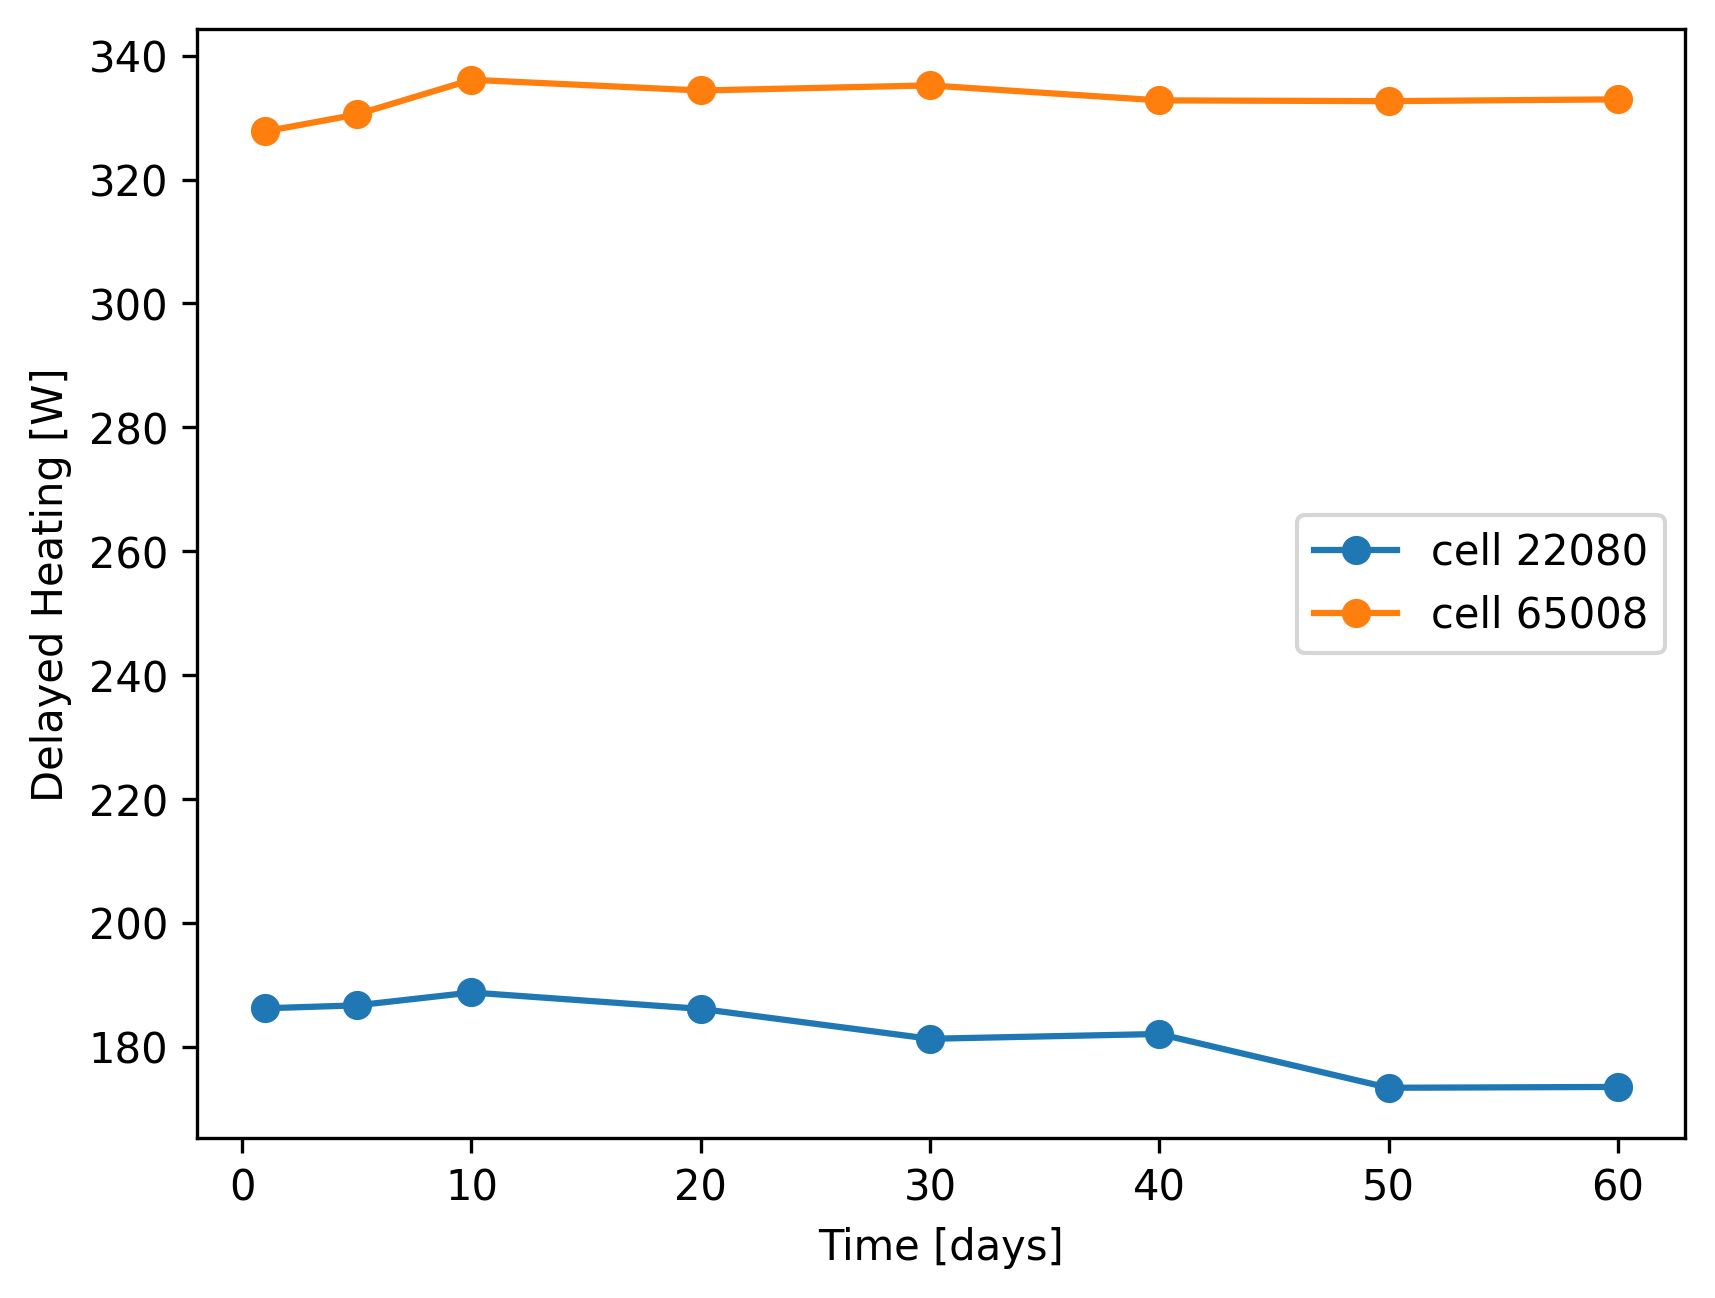
\includegraphics[width=0.90\linewidth]{figures/dh-bu-res3}
%   \end{center}
%   \caption{Delayed heating vs burnup for A2 (cell 22080) and I5 (cell 65008) experiment position.}
%   \label{fig:dh-bu}
% \end{figure}

% \begin{figure}[htbp!] % or H
%   \centering
%   \begin{subfigure}[b]{0.49\textwidth}
%     \centering
%     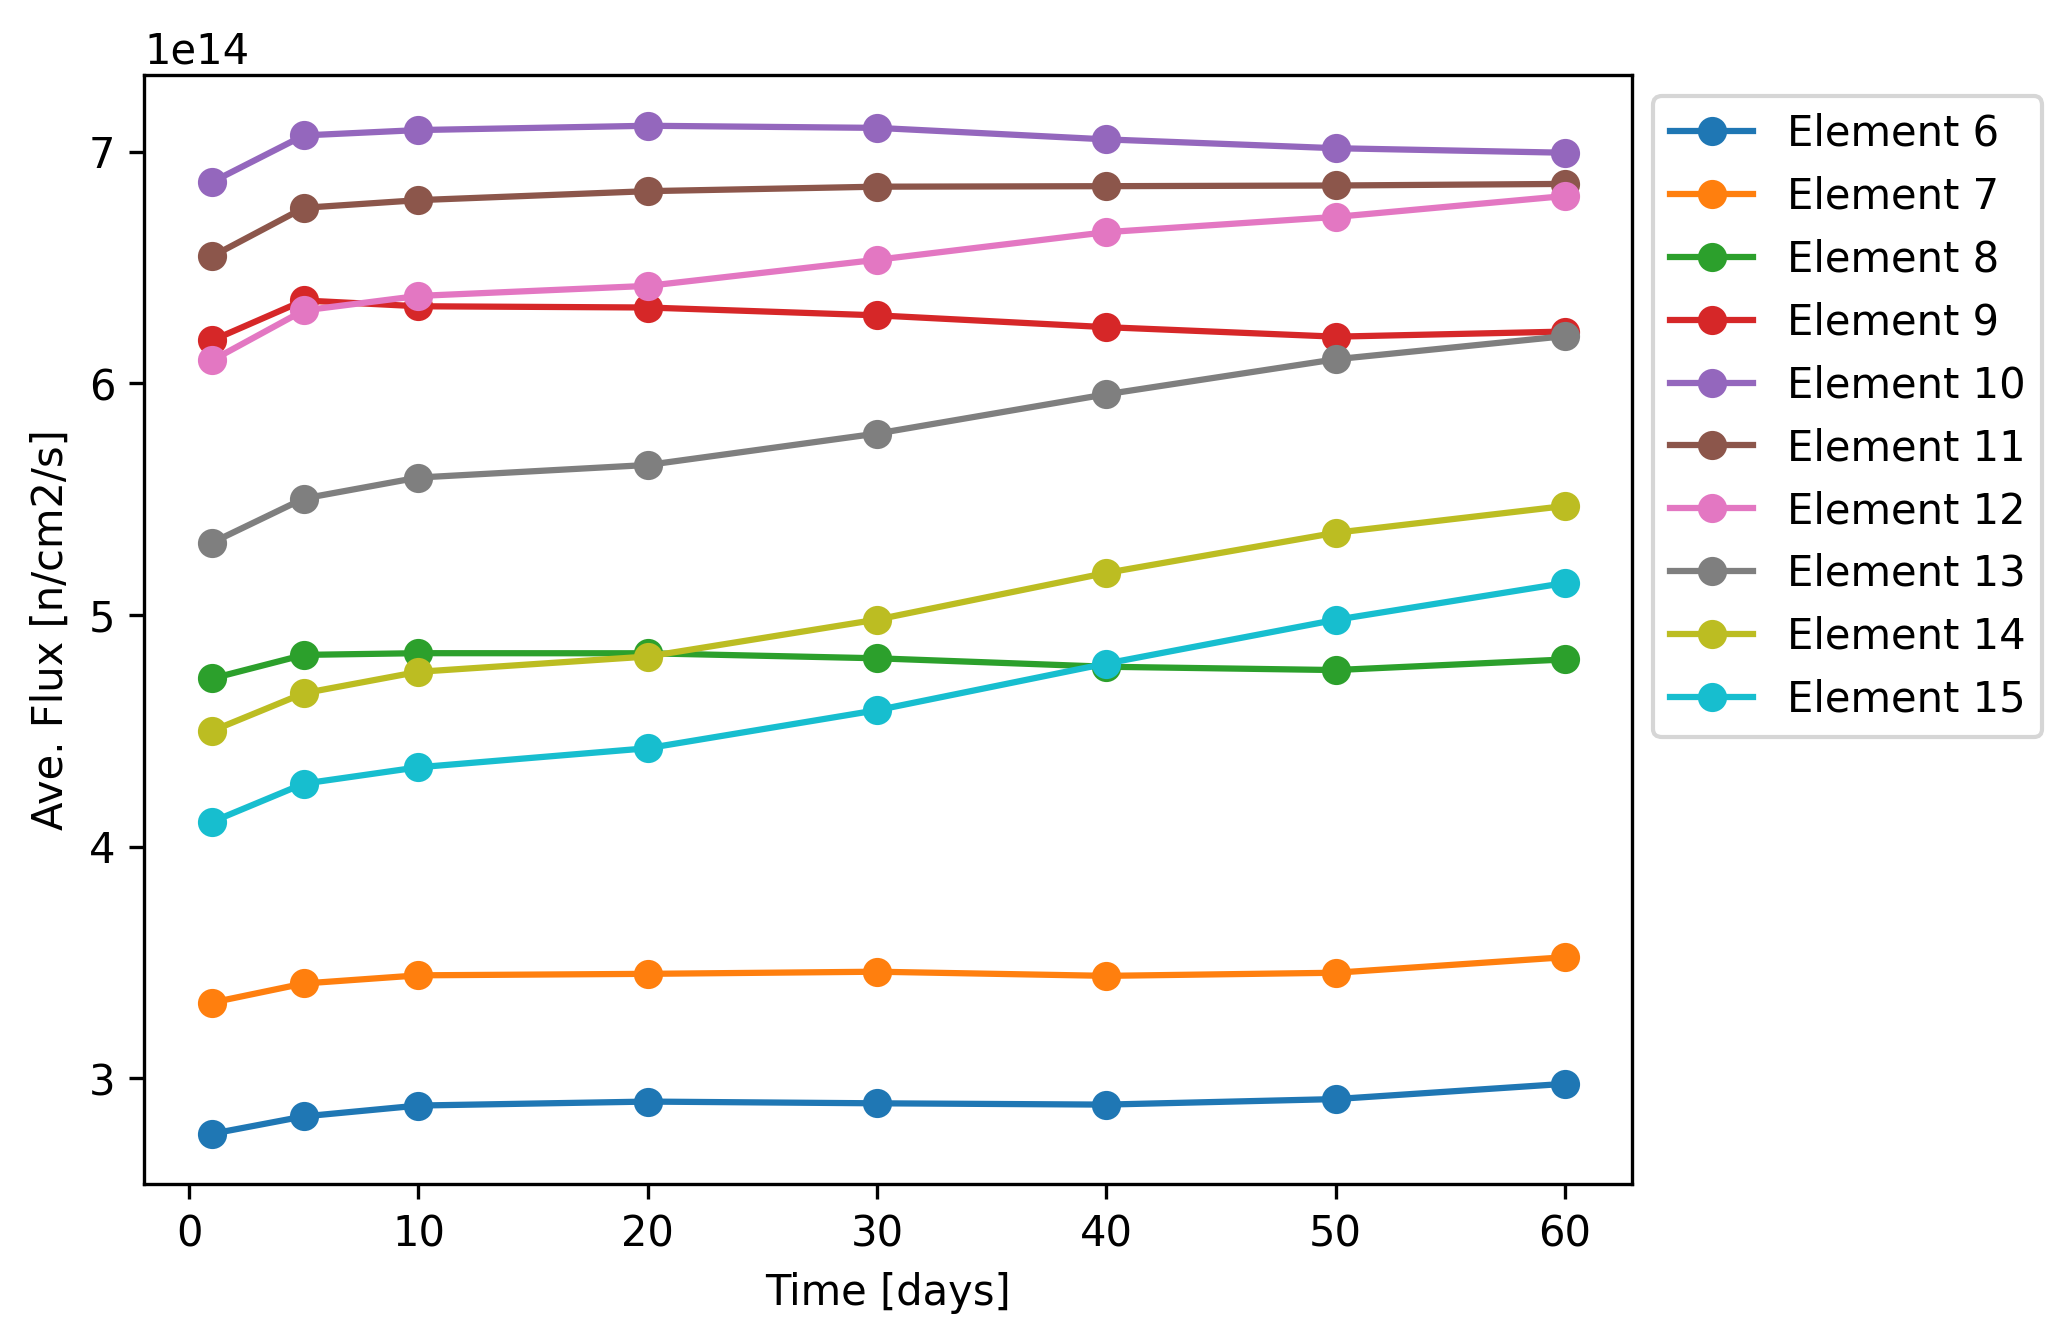
\includegraphics[width=0.7\textwidth]{figures/dh-bu-res1}
%     \caption{Average neutron flux.}
%   \end{subfigure}
%   \hfill
%   \begin{subfigure}[b]{0.49\textwidth}
%     \centering
%     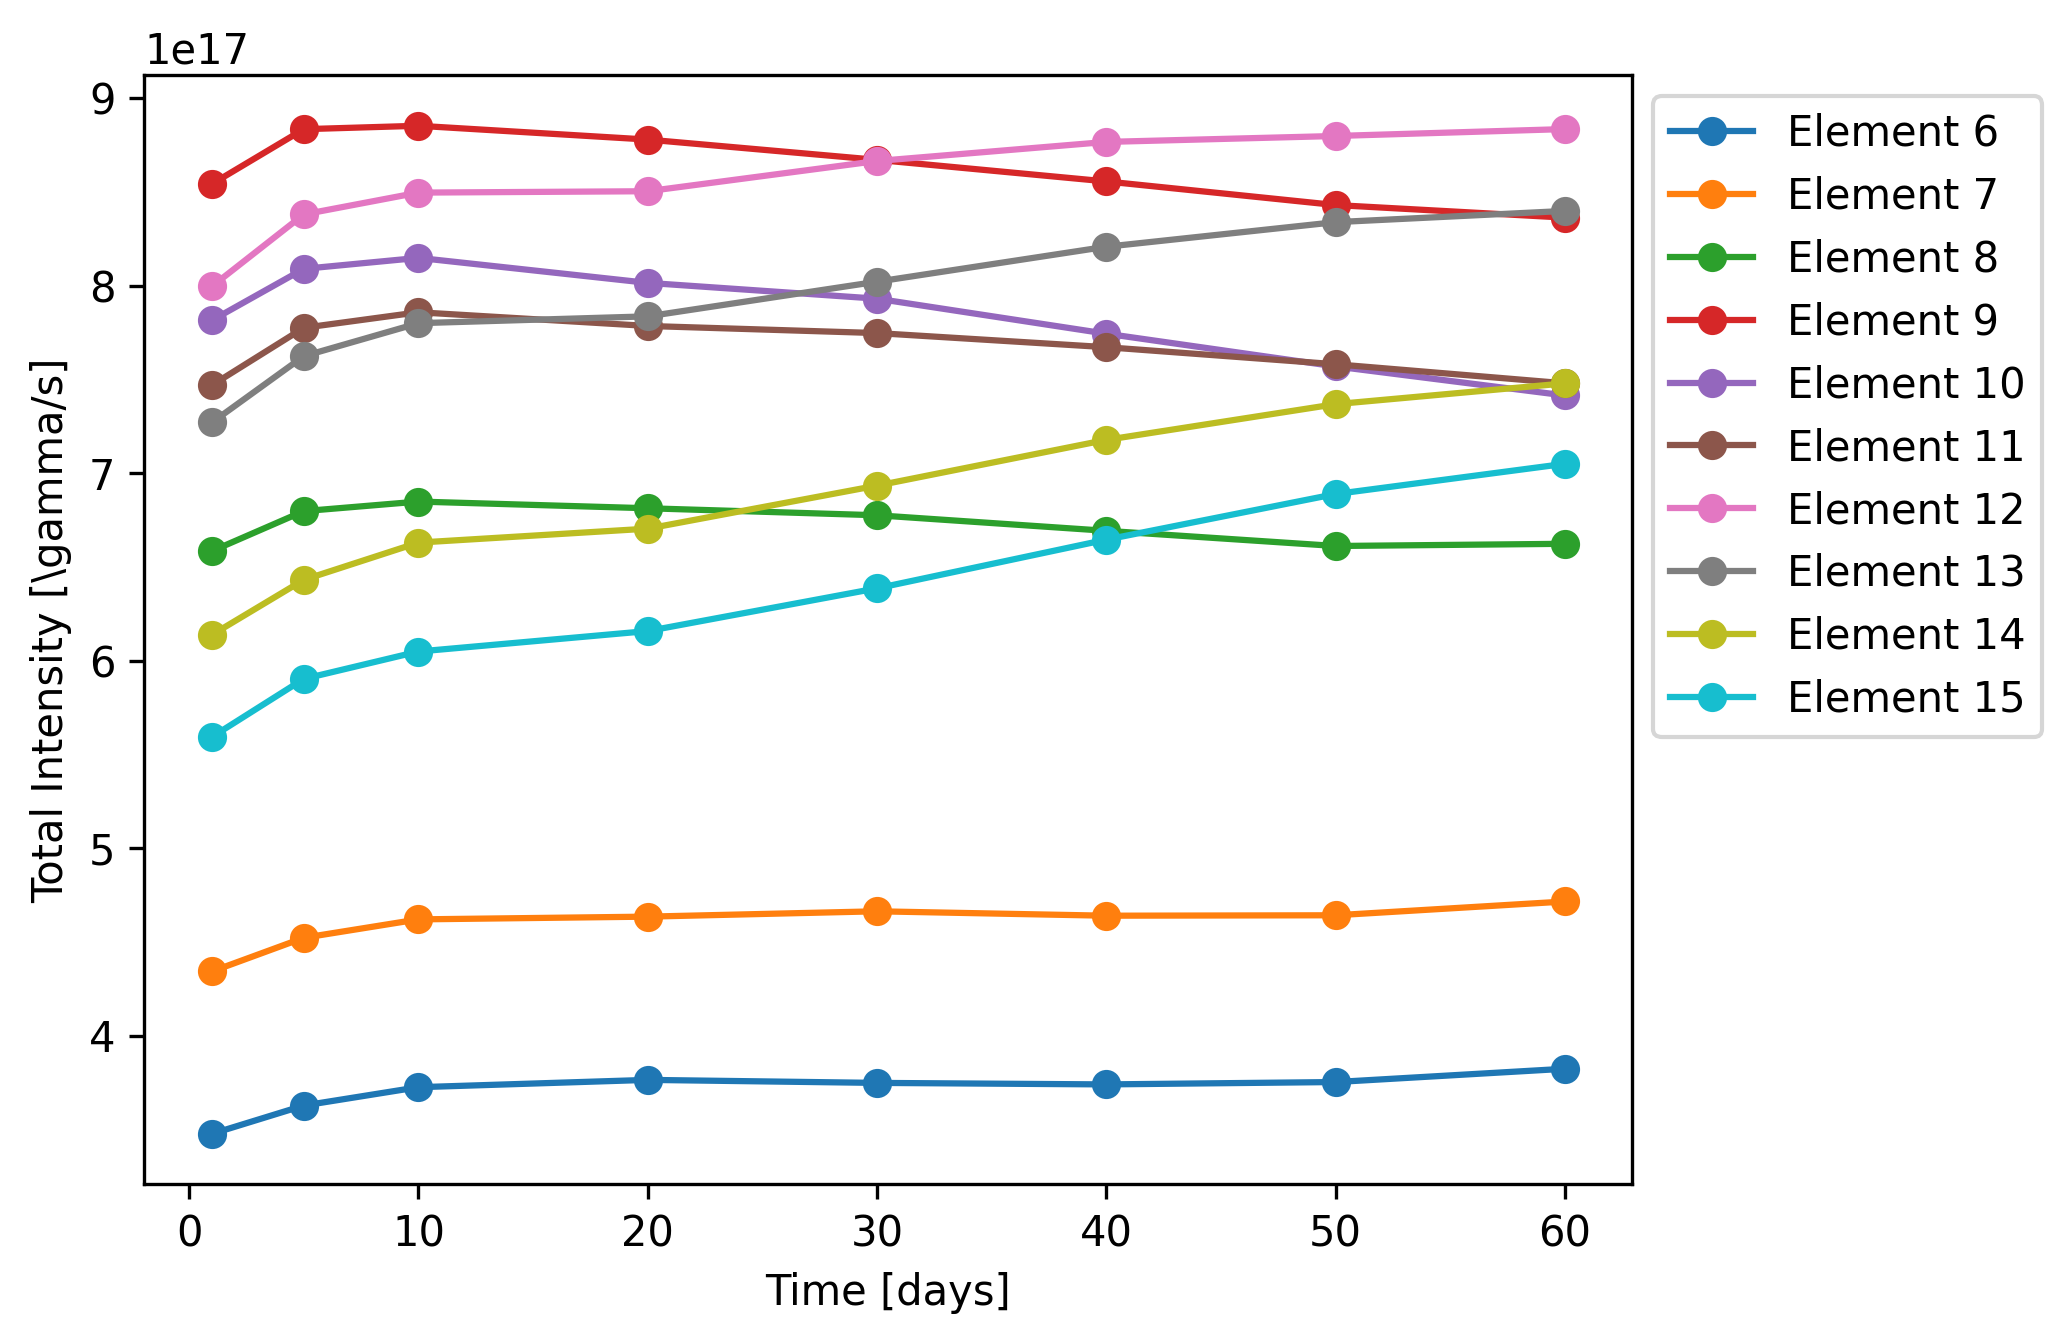
\includegraphics[width=0.7\textwidth]{figures/dh-bu-res2}
%     \caption{Total photon intensity.}
%   \end{subfigure}
%   \hfill
%   \caption{Magnitudes in the fuel assemblies closest to the experiment positions.}
%   \label{fig:flux-bu}
% \end{figure}

Figure \ref{fig:atr-data} displays $H_j(Z)$ and $H_j(\rho)$ for all the chemical elements included in the irradiation database.
$H_j(M)$ was plotted as well but the plot is not presented here.
As the relationship between $Z$ and $M$ is linear, the plots are very similar, and $H_j(M)$ does not convey any further information.
$H_{\gamma, Tr}(Z)$ increases with an increasing Z, but not monotonically.
For example, bromine (Z=35), cesium (Z=55), and mercury (Z=80) have lower heating values than the subsequent materials.
$H_{ch}(Z)$ does not present a clear trend with respect to Z.
The general trend for $H_j(\rho)$ is to increase with an increasing $\rho$.
This trend is clearer for the transported photon component than for the charged particle component.
$H_{ch}(\rho)$ is close to zero for densities smaller than 5 g/cm$^3$, has an increasing trend after 15 g/cm$^3$, and oscillates between 0 and 2 kW for the intermediate values.

\begin{figure}[htbp!] % or H
  \centering
  \begin{subfigure}[b]{0.49\textwidth}
    \centering
    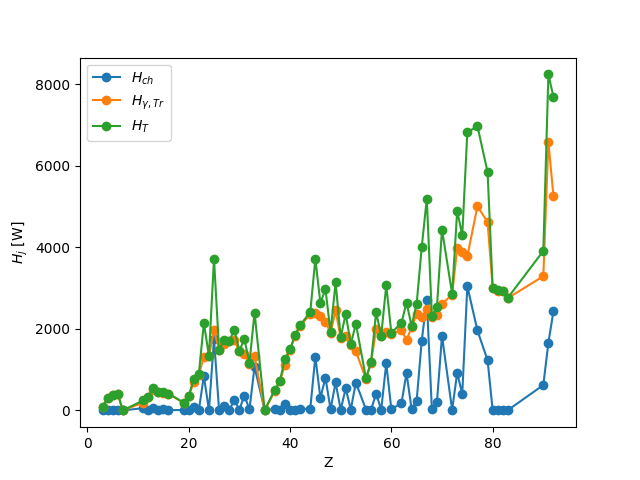
\includegraphics[width=0.95\textwidth]{figures/data-H_Z}
    \caption{$H_j(Z)$.}
  \end{subfigure}
  \hfill
  \begin{subfigure}[b]{0.49\textwidth}
    \centering
    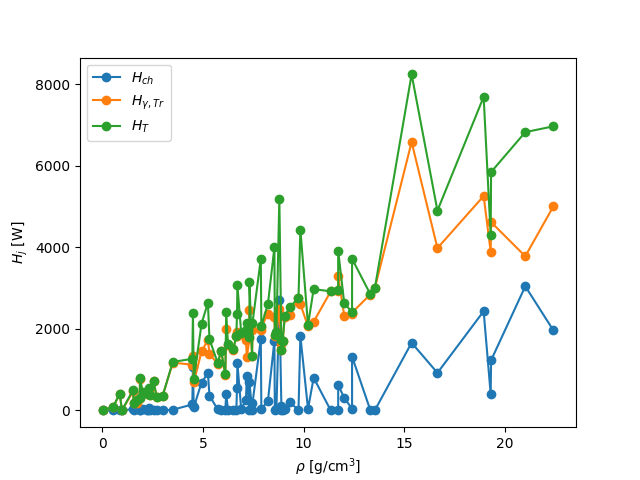
\includegraphics[width=0.95\textwidth]{figures/data-H_rho}
    \caption{$H_j(\rho)$.}
  \end{subfigure}
  \hfill
  \caption{Generic material irradiation database values for the ATR A1 experiment position.}
  \label{fig:atr-data}
\end{figure}

% Results from 14-
% Results
% Zircaloy-2
Figure \ref{fig:atr-time-zirc} presents the experiment heat production over time in an experiment of Zircaloy-2.
The reference curve is for an experiment of Zircaloy-2 with a density of 6.56 g/cm$^3$ and the following composition Zr-1.5Sn-0.15Fe-0.1Cr-0.05Ni.
The calculated curve corresponds to the results from the database method and are based on the delayed heating of samples of pure zirconium (7.13 g/cm$^3$), pure tin (5.75 g/cm$^3$), pure iron (7.87 g/cm$^3$), pure chromium (7.18 g/cm$^3$), and pure nickel (8.90 g/cm$^3$).
The delayed heating is 2.36 kW 1 second after shutdown, which is less than 0.01 \% of the total power during operation, and it decays below 500 W within 2 hours.
The calculated curve shows good agreement with the reference curve, having a relative difference smaller than 1\%.

\begin{figure}[htbp!] %or H 
    \centering
    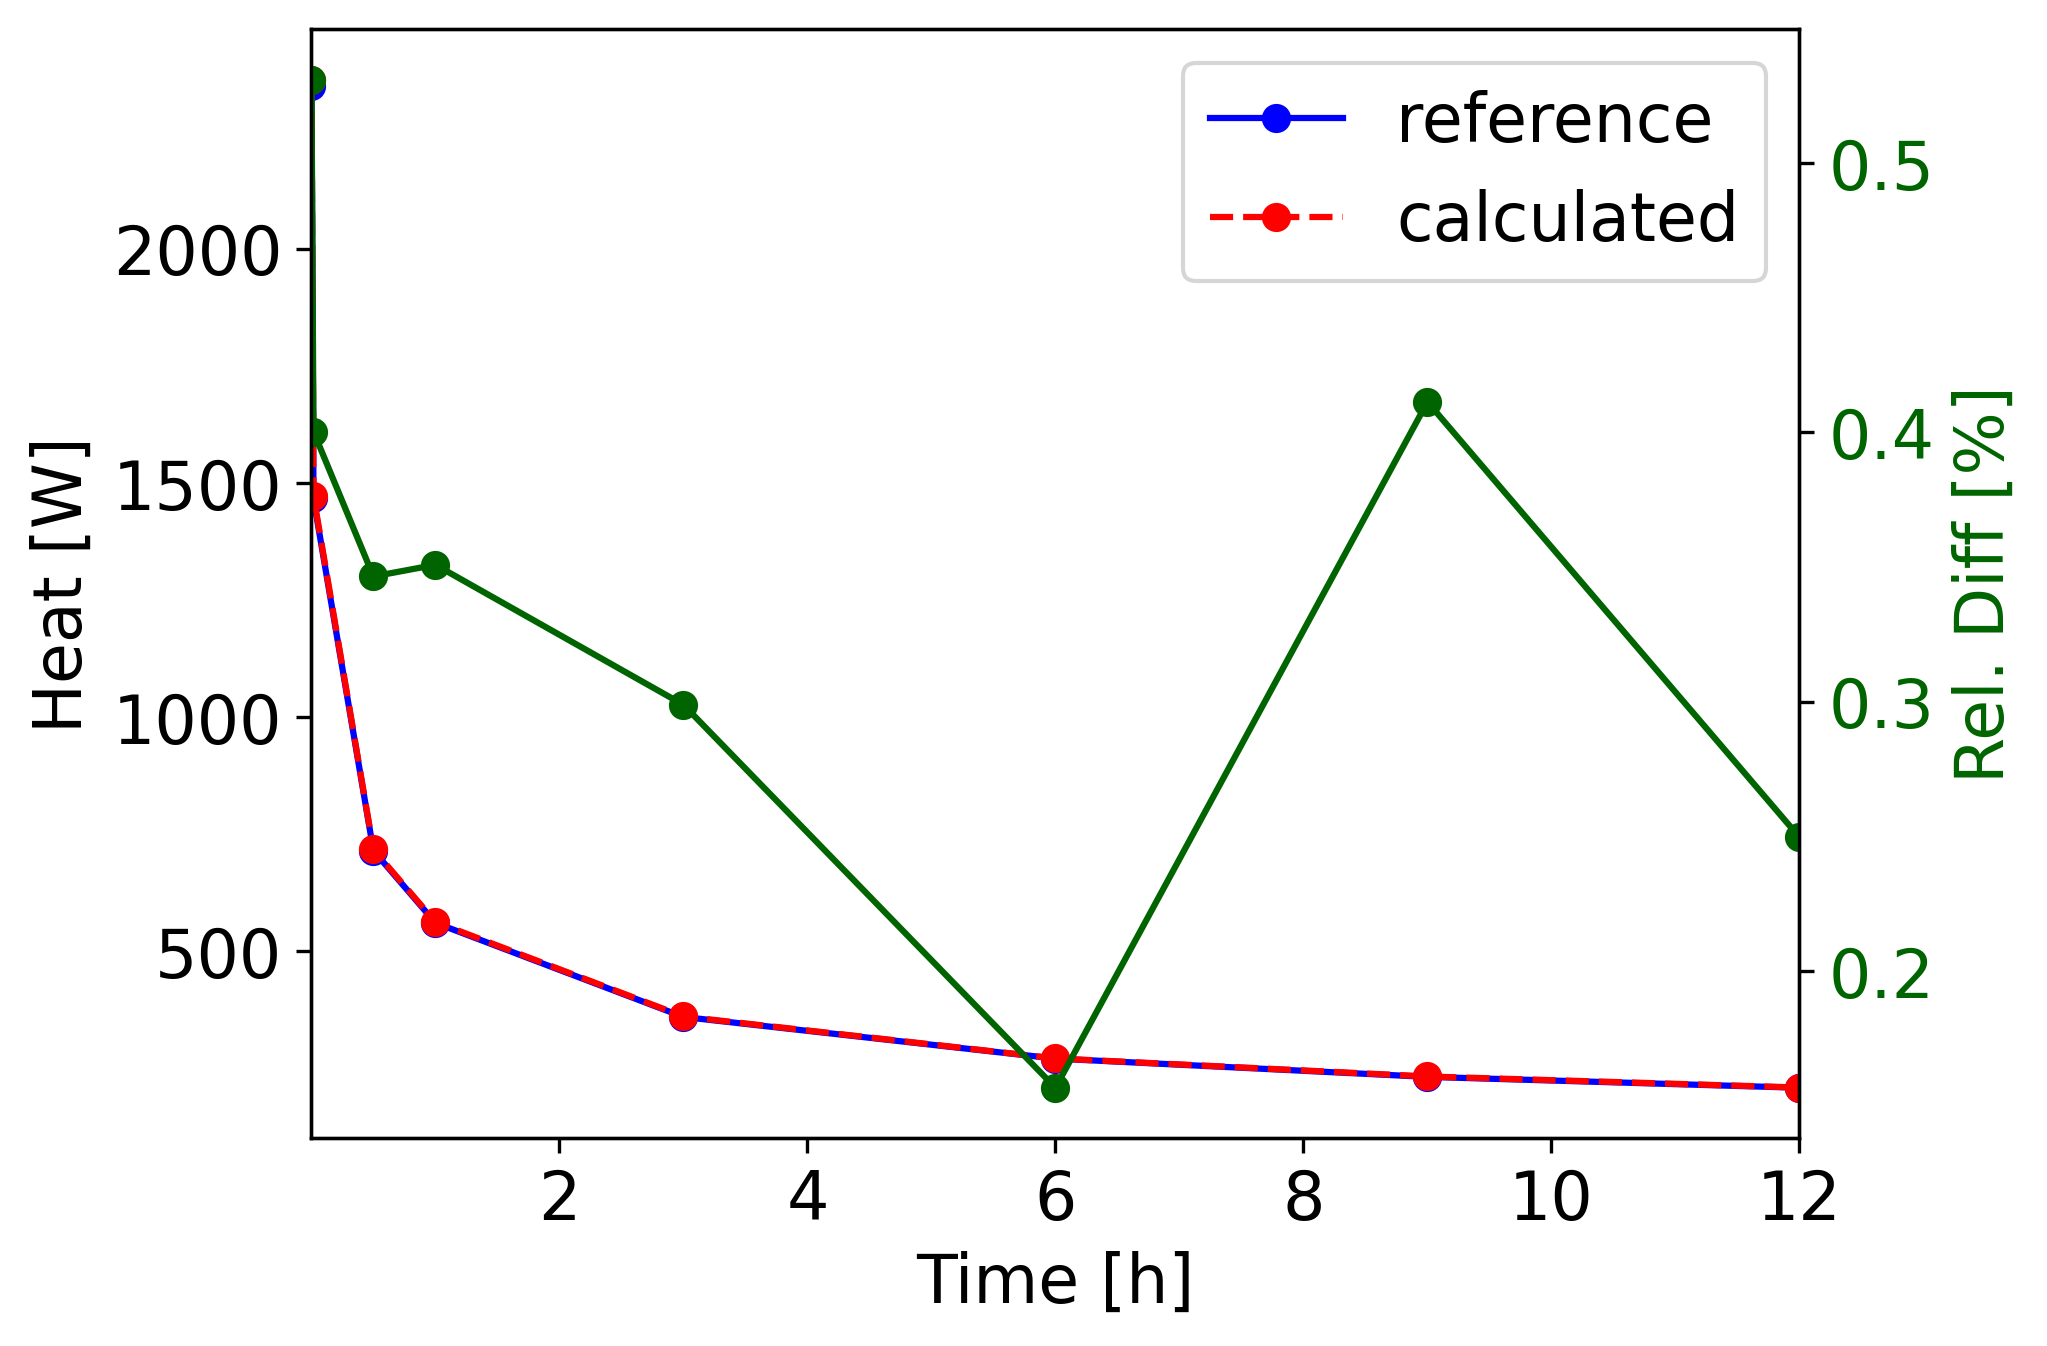
\includegraphics[width=0.60\linewidth]{figures/zircaloy2-tot-vs-t}
    \hfill
    \caption{Heat production over time in an experiment of Zircaloy-2.}
    \label{fig:atr-time-zirc}
\end{figure}

% decay step 0
% \begin{table}[htbp!]
%   \centering
%   \caption{.}
%   \label{tab:atr-zircaloy}
%   \begin{tabular}{cccc}
%     \toprule
%                     & \multicolumn{1}{c}{\begin{tabular}[c]{@{}c@{}}Database\\method [W]\end{tabular}} & \multicolumn{1}{c}{\begin{tabular}[c]{@{}c@{}}Reference\\calculation [W]\end{tabular}} & Rel. Diff [\%] \\
%     \midrule
%     \multicolumn{4}{c}{Zircaloy-2}                        \\
%     $H_{ch}$            &    2.95   &    2.96   & -0.10   \\
%     $H_{\gamma, Tr}$    & 2357.88   & 2345.41   &  0.53   \\
%     $H_{T}$             & 2360.83   & 2348.37   &  0.53   \\
%     \multicolumn{4}{c}{Zircaloy-4}                        \\
%     $H_{ch}$            &    2.95   &    2.96   & -0.29   \\
%     $H_{\gamma, Tr}$    & 2357.86   & 2345.63   &  0.52   \\
%     $H_{T}$             & 2360.82   & 2348.59   &  0.52   \\
%     \multicolumn{4}{c}{ZrNb}                              \\
%     $H_{ch}$            &    2.99   &    3.31   & -9.75   \\
%     $H_{\gamma, Tr}$    & 2307.60   & 2314.60   & -0.30   \\
%     $H_{T}$             & 2310.59   & 2317.92   & -0.32   \\
%     \bottomrule
%   \end{tabular}
% \end{table}

% FeCrAl
The following exercise considers an experiment of iron-chromium-aluminum (FeCrAl) alloy.
This type of alloy exhibits enhanced oxidation resistance in elevated temperature steam environments when compared to Zr-based alloys, making it a good cladding candidate for accident tolerant fuel in \glspl*{LWR} \cite{field_accident_2017}.
Additionally, it is stress corrosion cracking resistant and irradiation induced swelling resistant.
The typical content ranges from 10 to 22\% for chromium, and from 4 to 8\% for aluminum.
Figure \ref{fig:atr-time-fecral} presents the experiment heat production over time in the experiment of FeCrAl.
The reference curve is for an experiment of FeCrAl with a density of 8 g/cm$^3$ and the following composition Fe-22Cr-8Al.
The calculated curve corresponds to the results from the generic material irradiation database method and are based on the delayed heating of samples of pure iron (7.87 g/cm$^3$), pure chromium (7.18 g/cm$^3$), and pure aluminum (2.70 g/cm$^3$).
The delayed heating is 2.38 kW 1 second after shutdown, which is less than 0.01\% of the total power during operation, and it decays below 500 W within 2 hours.
The calculated curve shows good agreement with the reference curve, having a relative difference smaller than 1\%.

\begin{figure}[htbp!] %or H 
    \centering
    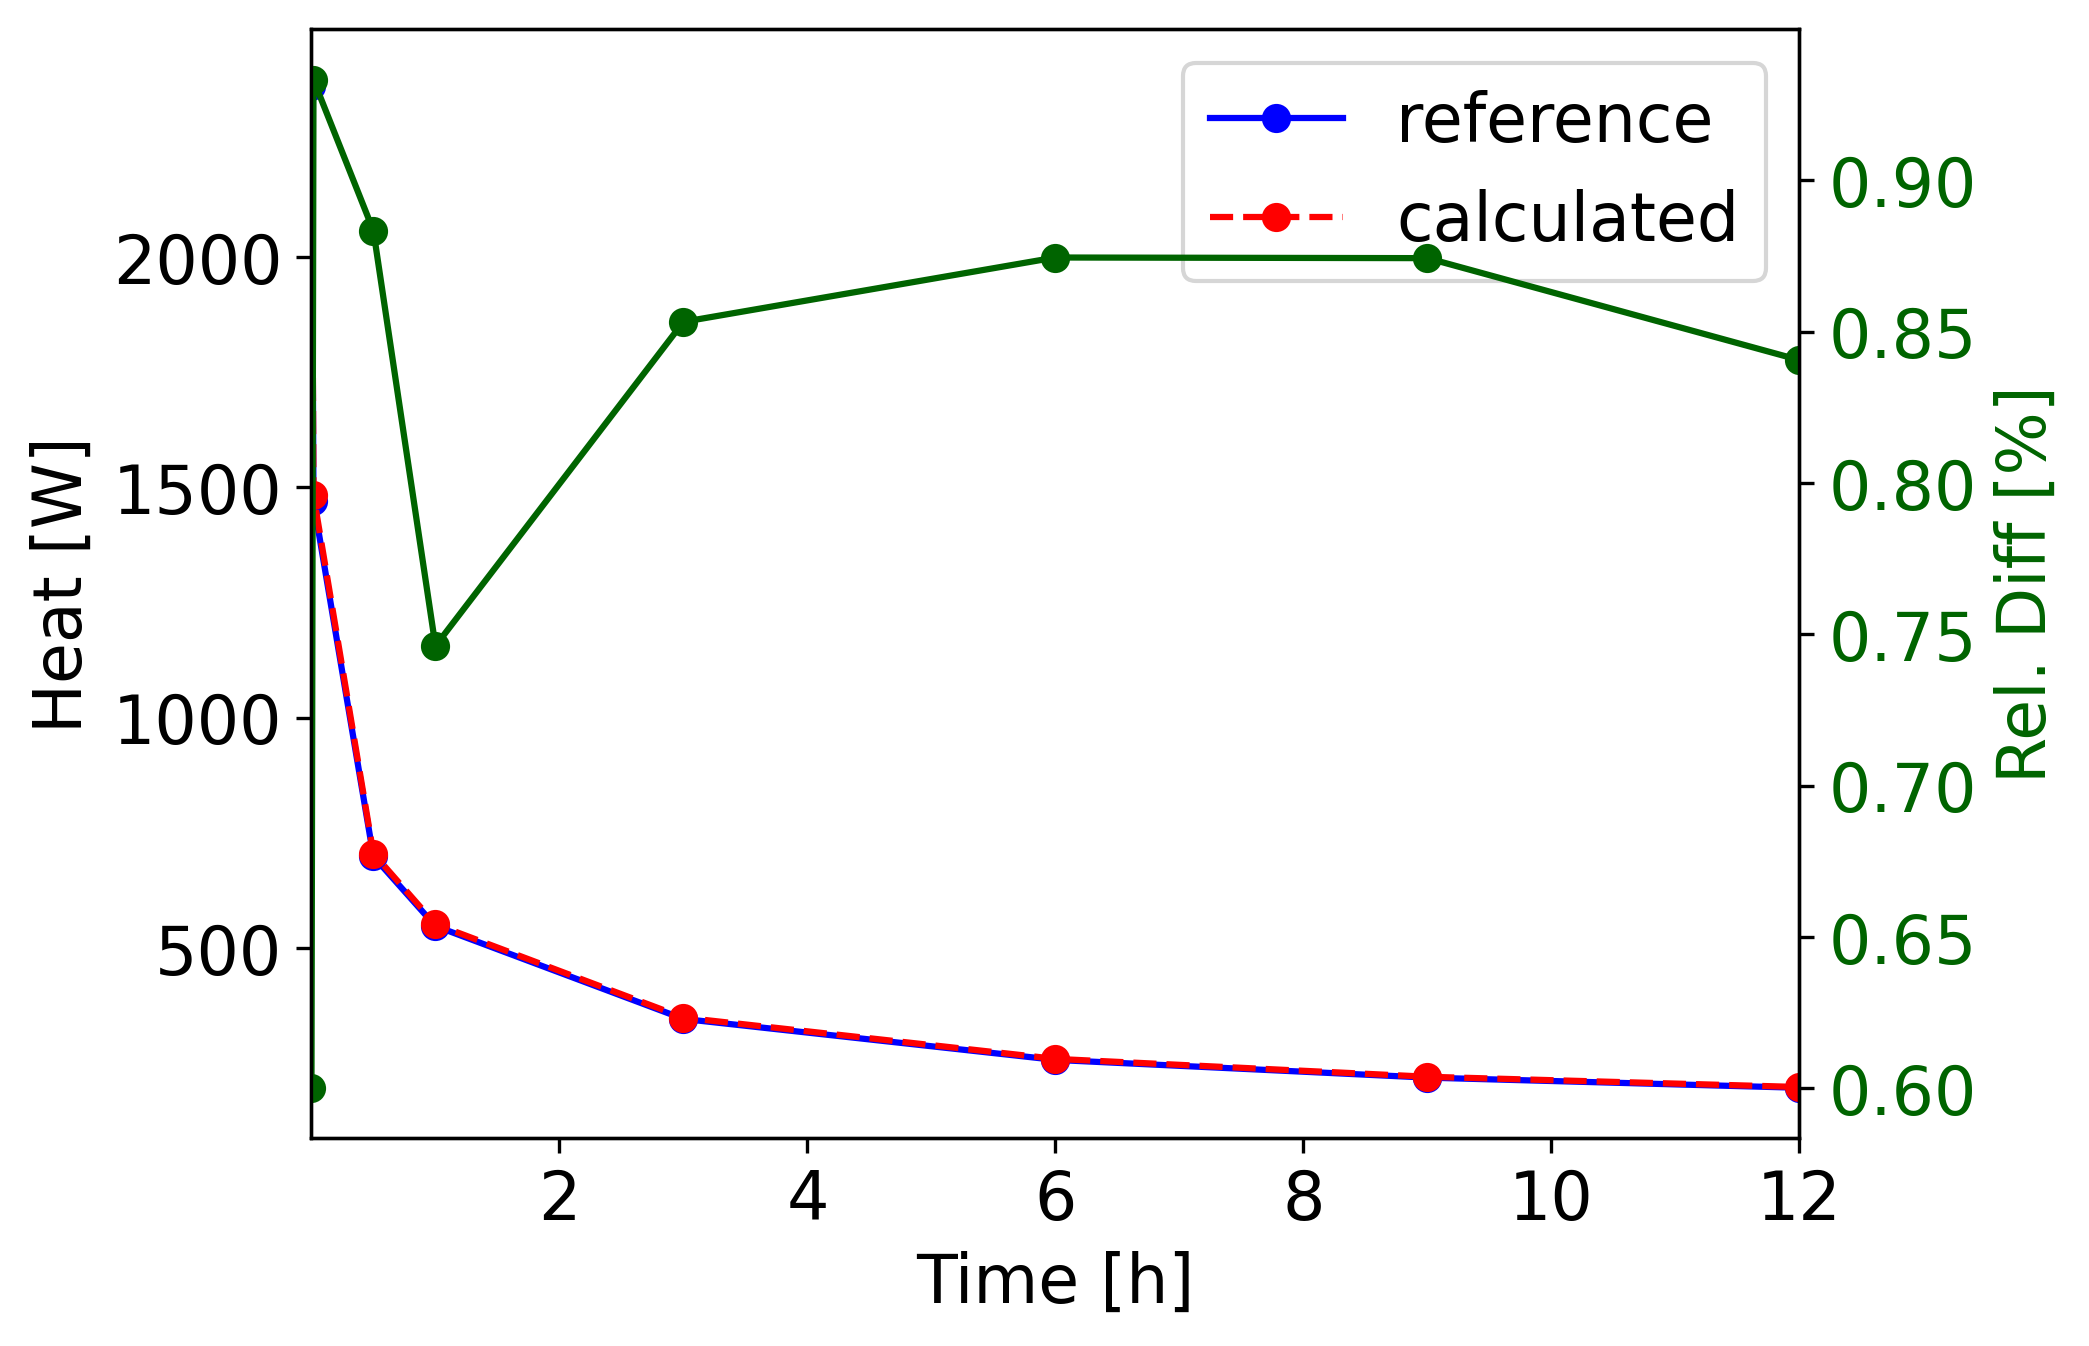
\includegraphics[width=0.60\linewidth]{figures/FeCrAl1-tot-vs-t}
    \hfill
    \caption{Heat production over time in an experiment of FeCrAl.}
    \label{fig:atr-time-fecral}
\end{figure}

% decay step 0
% \begin{table}[htbp!]
%   \centering
%   \caption{.}
%   \label{tab:atr-FeCrAl}
%   \begin{tabular}{cccc}
%     \toprule
%                     & \multicolumn{1}{c}{\begin{tabular}[c]{@{}c@{}}Database\\method [W]\end{tabular}} & \multicolumn{1}{c}{\begin{tabular}[c]{@{}c@{}}Reference\\calculation [W]\end{tabular}} & Rel. Diff [\%] \\
%     \midrule
%     \multicolumn{4}{c}{70\% Fe, 22\% Cr, 8\% Al}         \\
%     $H_{ch}$            &   14.87  &   12.21   & 21.80   \\
%     $H_{\gamma, Tr}$    & 2369.97  & 2358.40   &  0.49   \\
%     $H_{T}$             & 2384.84  & 2370.62   &  0.60   \\
%     \multicolumn{4}{c}{86\% Fe, 10\% Cr, 4\% Al}         \\
%     $H_{ch}$            &    7.57  &    6.24   & 21.39   \\
%     $H_{\gamma, Tr}$    & 2374.85  & 2367.56   &  0.31   \\
%     $H_{T}$             & 2382.42  & 2372.80   &  0.36   \\
%     \bottomrule
%   \end{tabular}
% \end{table}

% UMo
The following exercise considers an experiment of UMo with natural uranium.
Figure \ref{fig:atr-time-umo} presents the experiment heat production over time in the experiment of UMo.
The reference curve is for an experiment of UMo with a density of 17.35 g/cm$^3$.
The calculated curve corresponds to the results from the database method and are based on the delayed heating of samples of pure uranium and pure molybdenum.
The exercise adopts the following uranium densities for the calculations: 1, 7, 13, and 19 g/cm$^3$, and a molybdenum density of 10.22 g/cm$^3$.
The delayed heating is 11.29 kW 1 second after shutdown, which is 0.01 \% of the total power during operation, and it decays below 2 kW within 3 hours.
The calculated curve shows good agreement with the reference curve, having a relative difference of approximately 5\%.

\begin{figure}[htbp!] %or H 
    \centering
    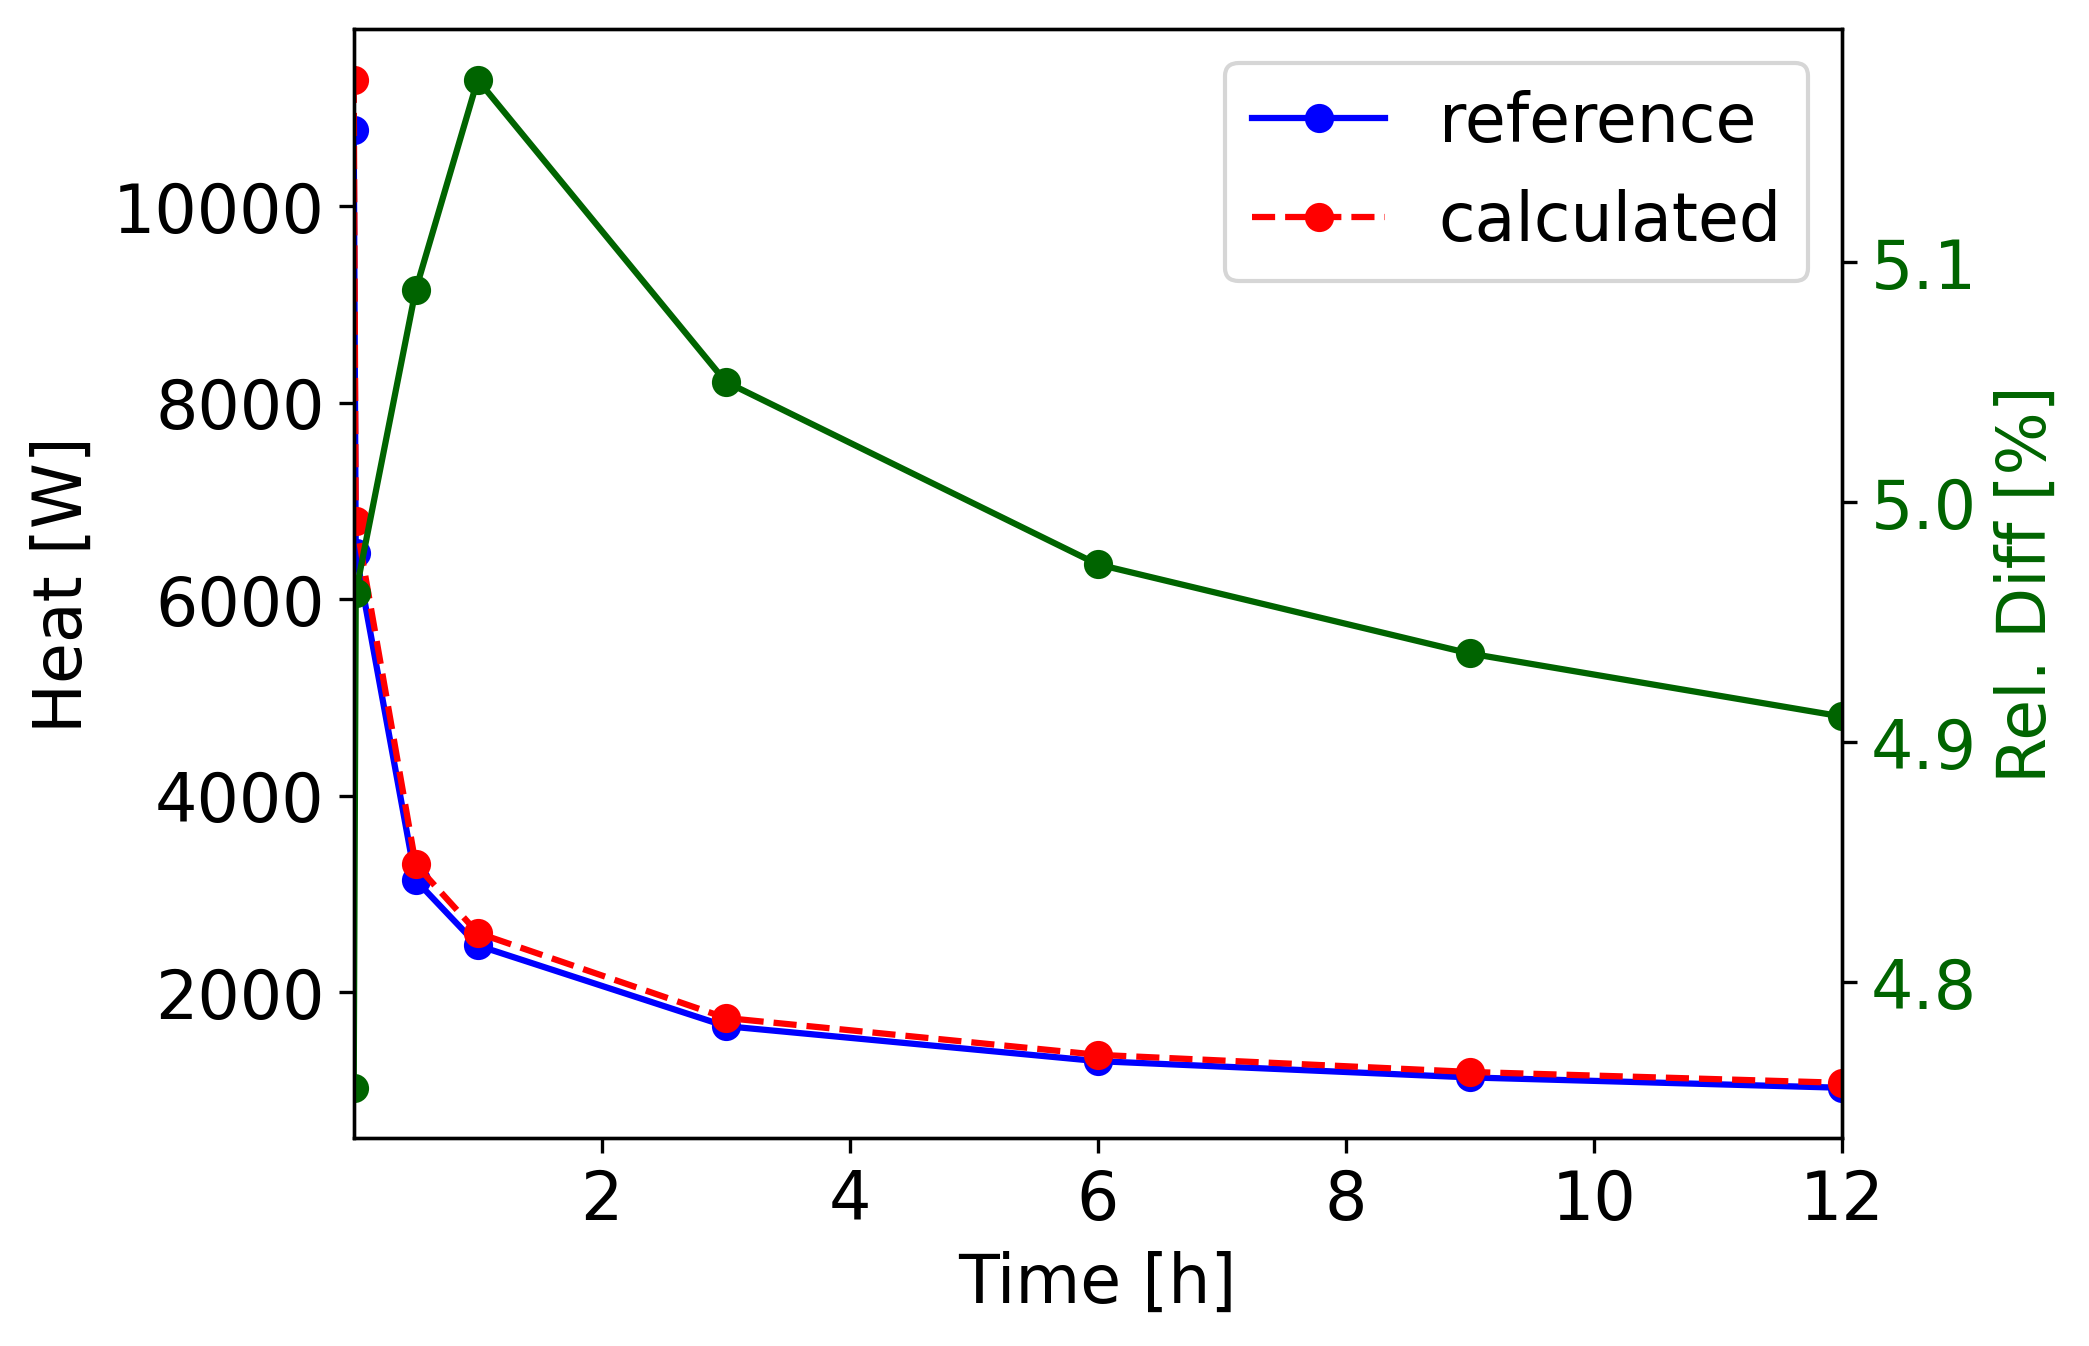
\includegraphics[width=0.60\linewidth]{figures/u-mo-tot-vs-t}
    \hfill
    \caption{Heat production over time in an experiment of UMo.}
    \label{fig:atr-time-umo}
\end{figure}

% decay step 0
% \begin{table}[htbp!]
%   \centering
%   \caption{.}
%   \label{tab:atr-Ualloys}
%   \begin{tabular}{cccc}
%     \toprule
%                     & \multicolumn{1}{c}{\begin{tabular}[c]{@{}c@{}}Database\\method [W]\end{tabular}} & \multicolumn{1}{c}{\begin{tabular}[c]{@{}c@{}}Reference\\calculation [W]\end{tabular}} & Rel. Diff [\%] \\
%     \midrule
%     \multicolumn{4}{c}{U(nat)-Mo}         \\
%     $H_{ch}$            &  3507.04   &  3416.95  &  2.64   \\
%     $H_{\gamma, Tr}$    &  7780.91   &  7358.50  &  5.74   \\
%     $H_{T}$             & 11287.95   & 10775.45  &  4.76   \\
%     \multicolumn{4}{c}{U(nat)-Nb}         \\
%     $H_{ch}$            &  3345.27   &  3306.49  &  1.17   \\
%     $H_{\gamma, Tr}$    &  7592.19   &  7156.94  &  6.08   \\
%     $H_{T}$             & 10937.46   & 10463.43  &  4.53   \\
%     \multicolumn{4}{c}{U(20\%)3Si2Al}     \\
%     $H_{ch}$            &  7783.68   &  7527.87  &  3.40   \\
%     $H_{\gamma, Tr}$    &  4690.24   &  4830.27  & -2.90   \\
%     $H_{T}$             & 12473.92   & 12358.14  & -0.94   \\
%     \bottomrule
%   \end{tabular}
% \end{table}


% % Other results
% The following analyses focus on the delayed heating over time for a mix of materials.
% % Bronze
% Figure \ref{fig:atr-time-brz} presents the experiment heat production over time in an experiment of bronze.
% The delayed heating is 2.97 kW 1 second after shutdown, which is less than 0.01 \% of the total power during operation, and it decays to 500 W after approximately 3 hours later.
% The calculated curve shows good agreement with the reference curve, having a relative difference smaller than 2\%.
% The reference curve is for an experiment of bronze with a density of 8.73 g/cm$^3$, and the weight fractions are 88\% and 12\% for copper and tin, respectively.
% The calculated curve corresponds to the results from the database method and are based on the delayed heating of samples of pure copper (8.96 g/cm$^3$) and pure tin (5.75 g/cm$^3$).

% \begin{figure}[htbp!] %or H 
%     \centering
%     \includegraphics[width=0.80\linewidth]{figures/bronze-tot-vs-t}
%     \hfill
%     \caption{Heat production over time in an experiment of bronze.}
%     \label{fig:atr-time-brz}
% \end{figure}

% % decay step 0
% % \begin{table}[htbp!]
% %   \centering
% %   \caption{.}
% %   \label{tab:atr-brz}
% %   \begin{tabular}{cccc}
% %     \toprule
% %                     & \multicolumn{1}{c}{\begin{tabular}[c]{@{}c@{}}Database\\method [W]\end{tabular}} & \multicolumn{1}{c}{\begin{tabular}[c]{@{}c@{}}Reference\\calculation [W]\end{tabular}} & Rel. Diff [\%] \\
% %     \midrule
% %     \multicolumn{4}{c}{Bronze}        \\
% %     $H_{ch}$            &  229.95   &  237.10  & -3.02  \\
% %     $H_{\gamma, Tr}$    & 2743.96   & 2754.34  & -0.38  \\
% %     $H_{T}$             & 2973.91   & 2991.44  & -0.59  \\
% %     \bottomrule
% %   \end{tabular}
% % \end{table}

% \begin{table}[htbp!]
%   \centering
%   \caption{.}
%   \label{tab:atr-sic}
%   \begin{tabular}{cccc}
%     \toprule
%                     & \multicolumn{1}{c}{\begin{tabular}[c]{@{}c@{}}Database\\method [W]\end{tabular}} & \multicolumn{1}{c}{\begin{tabular}[c]{@{}c@{}}Reference\\calculation [W]\end{tabular}} & Rel. Diff [\%] \\
%     \midrule
%     \multicolumn{4}{c}{SiC}        \\
%     $H_{ch}$            &    2.25  &    2.28  & -1.31  \\
%     $H_{\gamma, Tr}$    &  958.36  &  939.10  &  2.05  \\
%     $H_{T}$             &  960.60  &  941.38  &  2.04  \\
%     \bottomrule
%   \end{tabular}
% \end{table}

% \begin{table}[htbp!]
%   \centering
%   \caption{.}
%   \label{tab:atr-ss}
%   \begin{tabular}{cccc}
%     \toprule
%                     & \multicolumn{1}{c}{\begin{tabular}[c]{@{}c@{}}Database\\method [W]\end{tabular}} & \multicolumn{1}{c}{\begin{tabular}[c]{@{}c@{}}Reference\\calculation [W]\end{tabular}} & Rel. Diff [\%] \\
%     \midrule
%     \multicolumn{4}{c}{SS}        \\
%     $H_{ch}$            &   54.70  &   57.28  &  -4.51  \\
%     $H_{\gamma, Tr}$    & 2401.44  & 2402.40  &  -0.04  \\
%     $H_{T}$             & 2456.14  & 2459.68  &  -0.14  \\
%     \bottomrule
%   \end{tabular}
% \end{table}

% \begin{table}[htbp!]
%   \centering
%   \caption{.}
%   \label{tab:atr-w}
%   \begin{tabular}{cccc}
%     \toprule
%                     & \multicolumn{1}{c}{\begin{tabular}[c]{@{}c@{}}Database\\method [W]\end{tabular}} & \multicolumn{1}{c}{\begin{tabular}[c]{@{}c@{}}Reference\\calculation [W]\end{tabular}} & Rel. Diff [\%] \\
%     \midrule
%     \multicolumn{4}{c}{95\%-W, 3.5\%-Ni, 1.5\%-Fe}      \\ % Double check the composition
%     $H_{ch}$            &  310.55  &  329.49  & -5.75   \\
%     $H_{\gamma, Tr}$    & 5463.04  & 5671.29  & -3.67   \\
%     $H_{T}$             & 5773.59  & 6000.78  & -3.79   \\
%     \bottomrule
%   \end{tabular}
% \end{table}

% \begin{table}[htbp!]
%   \centering
%   \caption{.}
%   \label{tab:atr-RAFM}
%   \begin{tabular}{cccc}
%     \toprule
%                     & \multicolumn{1}{c}{\begin{tabular}[c]{@{}c@{}}Database\\method [W]\end{tabular}} & \multicolumn{1}{c}{\begin{tabular}[c]{@{}c@{}}Reference\\calculation [W]\end{tabular}} & Rel. Diff [\%] \\
%     \midrule
%     \multicolumn{4}{c}{RAFM}         \\
%     $H_{ch}$            &    9.01  &   12.66  & -28.83   \\
%     $H_{\gamma, Tr}$    & 2381.76  & 2369.79  &   0.51   \\
%     $H_{T}$             & 2390.77  & 2382.45  &   0.35   \\
%     \bottomrule
%   \end{tabular}
% \end{table}

\section{Conclusions}

% From 14-
% Intro
Safety analyses in research reactors require the estimation of heat deposited in experiments and reactor structures after shutdown.
Research reactors enable the irradiation of a wide variety of unique experiments, requiring the development of safety analyses on a case-by-case basis, which often proves to be effort- and time-consuming.
This chapter studies two methods using previous knowledge to expedite the process.

First, the chapter investigates the feasibility of reducing the calculation burden by solving the neutron-transport problem only once.
This fast method utilizes the geometry-dependent parameters from the neutron-transport problem for an experiment of carbon, which is a material that does not considerably perturb the neutron flux.
Then, the depletion calculation utilizes these parameters to obtain the charged particle heating and photon source intensity.
Some cases are studied for selected materials and the results compared to the results obtained with the delayed heating calculation workflow.
The results show that the fast calculation is accurate for some cases while excessively conservative for others.
Additionally, the study concludes that this approach is not suitable to this thesis' objectives and that neutron-transport simulations cannot be avoided.

Second, this chapter also describes the generic material irradiation database method, which relies on the delayed heating calculation to obtain the heat produced in experiments of individual chemical elements and through their combination calculate the heat produced in experiments of arbitrary material composition.
% Results
Finally, this chapter demonstrates the generic material irradiation database method by presenting two exercises.
These exercises include the delayed heating calculation of experiments for a demonstration exercise and ATR.
The results verify the method by showing a wide variety of combinations of materials that could integrate a research reactor experiment.
Additionally, for the case of the ATR exercise, the heat production over time is shown for several experiments.
Overall, the results exhibit good agreement between the calculated and reference values.

% Future work
% Further investigation is needed to understant the perfomance of this method on experiments comprising a mix of heavy/fissile elements. 